\begin{resume}
Dans l'ensemble des éléments qui composent les systèmes informatiques, le réseau d'interconnexion est parmi les éléments qui sont les plus exposés et impactés par l'hétérogénéité. Cette hétérogénéité peut se présenter sous différentes formes : diversité d'équipements et de technologies, variations de performance et disponibilité (volatilité), limitations liées aux caractéristiques physiques ou à la capacité des ressources, etc. 

Si cette hétérogénéité doit être prise en compte lors du développement de systèmes et applications, il s'avère souvent que les solutions se limitent à pallier les éventuels problèmes. Les travaux que j'ai mené dans le domaine de l'hétérogénéité des réseaux visent la compréhension des facteurs liés à l'hétérogénéité, leur caractérisation et aussi l'optimisation de l'usage des ressources afin de rendre les systèmes et applications plus performants et fiables.

L'une des premières étapes dans l'étude de l'hétérogénéité requiert l'observation et l'analyse des communications réseau afin de modéliser leur fonctionnement et ainsi permettre une estimation de leurs performances. Cette étude cache néanmoins une grande complexité car même sur un petit ensemble de ressources la variation de certains facteurs peut créer un nombre important de situations, chacune avec un modèle de communication différent. Afin de permettre l'application pratique de cette modélisation de performance nous devons non seulement être en mesure de découvrir la topologie du réseau, mais aussi de pouvoir quantifier les différents facteurs et émettre des hypothèses sur les modèles de communication observés. 

Un mécanisme très utile dans la réduction de la complexité de la modélisation des communications réside dans la classification et catégorisation des ressources observées. Non seulement cela permet de se concentrer sur des modèles "type" qui représentent convenablement des ensembles de ressources, comme aussi on ouvre la possibilité d'utiliser ces informations dans le but d'optimiser les échanges entre les applications.

Tous ces éléments sont connectés aux travaux qui seront présentés dans les chapitres suivants.  
%Cette première partie regroupe les travaux que j'ai menés sur la
%structuration des systèmes distribués à l'aide de marches
%aléatoires. Ils constituent la continuité de ceux menés durant ma
%thèse.
%
%J'exploite les marches aléatoires selon deux axes. Le premier consiste
%à n'utiliser que la circulation, sans collecte d'informations au cours
%du déplacement. Le second consiste à combiner les concepts de marche
%aléatoire et de mot circulant, afin d'exploiter l'historique des
%déplacements du jeton.
%
%La première approche m'a permis de définir un algorithme rapide de
%construction et de maintenance d'un arbre couvrant sur un système
%distribué. Cette construction est auto-stabili\-sante, et garantit
%donc la tolérance aux fautes transitoires qui peuvent affecter le
%système.
%
%Dans la seconde approche, l'historique des déplacements est conservé
%dans le jeton, mais n'a aucun impact sur la circulation qui reste
%aléatoire sans mémoire. Le contenu du jeton est analysé et exploité,
%afin de permettre la construction d'arbres couvrants sur chaque
%site. Je propose différents algorithmes auto-stabilisants de gestion
%et de correction du contenu du jeton et de sa circulation. Je dérive
%de cette circulation un algorithme auto-stabilisant garantissant la
%$k-$exclusion mutuelle.
%
%La majorité des travaux présentés dans cette partie, ont été réalisés
%en collaboration avec Alain Bui, professeur à l'université de Reims
%Champagne-Ardenne, et Thibault Bernard, dont je co-encadre une partie
%des travaux de thèse avec Alain Bui.

\end{resume}

\section{Modélisation des Performances d'un Réseau\label{sec:reseaux-model}}

%Dans le contexte de la modélisation de performance, nous appelons
%modèle la description formelle de l'exécution d'un programme sur une
%ou plusieurs machines, de manière à ce que cette description peut
%être utilisée pour comprendre, voire décrire, la performance de tel
%programme.

Une des meilleures manières de comprendre le fonctionnement des algorithmes
distribués et d'évaluer leur efficacité est de modéliser la performance
de ces algorithmes. Si d'un côté des facteurs non
déterministes influencent la performance des applications,
comme par exemple la congestion des ressources, pour la plupart du
temps leur impact sur le temps d'exécution est suffisamment
limité \cite{Grove03}. Ainsi, la plus grande difficulté pour la modélisation
des performances est la correcte représentation des facteurs liés
à la communication.  

Si les principes de la modélisation de performance peuvent être trouvés
dans des travaux pionniers des années 60 et 70 \cite{Peterson81},
la modélisation de performance a connu une importante attention à
partir des années 80, où des efforts importants ont été faits pour
identifier des modèles de performance adaptés aux technologies et
paradigmes qui ont surgi depuis la décennie précédente. Pour cette
raison, dans ce chapitre nous voulons identifier les modèles qui ont les caractéristiques
les plus adaptées à la modélisation réaliste des communications.


\subsection{Exécution dans les systèmes distribués}

Un système distribué est classiquement défini comme un ensemble
d'unités de traitement ou de calcul indépendantes, reliées entre elles
par des liens de communications. Ces unités de traitement contribuent
au calcul d'un résultat en effectuant leurs exécutions de façon
concurrente.

Un réseau d'interconnexion {\cal R}, aussi appelé système distribué,
est représenté par un graphe $G =(V,E)$, dans lequel $V$ est
l'ensemble des n{\oe}uds et $E$ l'ensemble des arêtes. Les n{\oe}uds
du graphe représentent les sites du réseau, les arêtes du graphe les
liens, ou canaux de communication du réseau.

Par la suite, on parlera indifféremment de n{\oe}ud, de site, de
processus ou de processeur pour définir un n{\oe}ud du réseau. De
même, on parlera indifféremment de canaux ou de liens de communication
pour définir les supports de la communication qu'utilise le réseau.

L'écriture d'un algorithme, ainsi que l'évaluation de ses
performances, ne peut se faire que si l'on a, au préalable, défini un
modèle d'exécution. La modélisation sert à imposer les contraintes
permettant de se rapprocher de la réalité. Les algorithmes distribués
sont écrits selon trois modèles principaux : le modèle à états, le
modèle à registres et le modèle à passage de messages.

Le modèle à états a été défini par Dijkstra \cite{Dij74}. Les sites ne
communiquent pas par l'intermédiaire d'échanges de messages, mais par
leur capacité à lire l'état de la mémoire de leurs voisins. Un site
accède en lecture et en écriture à l'ensemble de son environnement et
aux variables qu'il détient, mais il accède uniquement en lecture à
l'environnement de ses voisins.

Le modèle à registres partagés représente les liens de communication
comme des registres attachés à chaque site. Un lien $l_{ij}$ reliant
les sites $i$ et $j$ "porte" donc un registre $R_{ij}$ dans lequel
le site $i$ écrit les informations à transmettre au site $j$. De même,
il existe un registre $R_{ji}$ utilisé par le site $j$ pour
transmettre des informations au site $j$.

Le modèle à passage de messages définit des canaux de communication
par lesquels transitent les messages. Il nécessite de poser des
hypothèses sur les propriétés des canaux de communication : taille,
délais de transmission, caractéristiques des échanges...

Les différents modèles permettent une approche progressive des
communications dans les systèmes distribués. Lynch \cite{Lyn96}
propose toutefois des algorithmes et des méthodes permettant de
transformer un algorithme écrit pour un modèle à registres partagés en
un algorithme exploitant le modèle à passage de messages.

Dans notre cas spécifique, nous voulons explorer le modèle à passage de messages,
étudiant notamment les modèles de performance qui peuvent apporter à la fois une
représentation fidèle du comportement des communications mais aussi une 
utilisation simple, capable d'être appliquée sur des environnements hétérogènes.

%\subsection{Hockney}
%
%Le modèle de Hockney \cite{Hockney94} est un des plus utilisés pour
%décrire la communication point-à-point dans les machines parallèles
%à mémoire distribuée. Selon ce modèle, une communication entre deux
%noeuds est décrite par : 
%
%\[
%t=t_{0}+\frac{m}{r_{\infty}}\]
%
%
%où $t_{0}$ représente le temps nécessaire à l'envoi d'un message
%de taille zéro, \emph{m} est la taille du message (en octets) et $r_{\infty}$
%est le débit asymptotique en Moctets/s, i.e., le débit maximal obtenu
%quand la taille du message s'approche de l'infini. Dans ce raisonnement,
%$m/r_{\infty}$ représente le délai de transmission d'un message de
%\emph{m} octets à travers un réseau avec un débit asymptotique de
%$r_{\infty}$ Moctets/s.
%
%Ce modèle est souvent transformé dans l'équation affine 
%
%\[
%t=\alpha+\beta m\]
%
%
%où $\alpha$ correspond à la latence de transmission et $\beta$ est
%le temps de transfert d'un octet sur ce réseau \cite{Pjesivac-Grbovic05}.
%L'obtention des paramètres $\alpha$ et $\beta$ peut se faire à travers
%l'utilisation de certains outils comme NWS \cite{Wolski97}. 
%
%Toutefois, un inconvénient de ce modèle est qu'il assume que le temps
%de transfert est proportionnel à la taille du message. Dans des situations
%réelles, certains facteurs comme la taille de la mémoire tampon et
%la segmentation des messages en paquets font varier le temps de transfert
%$\beta$ selon la taille du message. 
%
%\subsection{Postal}
%
%À partir de l'observation qu'un des principaux paramètres pour la
%modélisation des algorithmes parallèles est le coût de communication
%entre les processus, Bar-Noy et Kipnis ont proposé le modèle Postal
%\cite{Bar-Noy94}. Le modèle Postal est fondé sur un paramètre $\lambda=t_{u}/t_{snd}$,
%où $t_{snd}$ est le temps nécessaire à un processus pour envoyer
%un message (la latence d'envoi), alors que $t_{u}$ représente le
%temps total nécessaire à la réception du message par le processus
%destinataire. Une des innovations du modèle Postal par rapport à ses
%prédécesseurs est que ce modèle permet des situations où un processus
%peut émettre plusieurs messages avant que le premier récepteur a reçu
%son message : cela est dû à une analogie avec l'envoi de lettres par
%la poste. 
%
%Prenons par exemple le cas d'une diffusion ou \emph{broadcast}. Par
%simplicité, il est considéré que $\lambda$ est une valeur entière
%et que le temps est mesuré en cycles, dont la durée est équivalente
%à la latence d'envoi d'un message. Dans le cas du \emph{Broadcast},
%la valeur de $\lambda$ influence la forme de l'arbre de diffusion
%qui permet la meilleure performance. C'est ainsi que la Figure \ref{Figure:Postal Model}
%compare deux arbres de diffusion différents, chacun contenant huit
%noeuds et $\lambda=2$. On observe que l'arbre binomial, (Figure \ref{Figure:Postal Model}a),
%malgré son optimalité quand $\lambda=1$, nécessite six étapes de
%communication pour compléter l'opération, alors que l'arbre représenté
%dans la Figure \ref{Figure:Postal Model}b nécessite seulement cinq
%étapes. En effet, la construction de l'arbre de diffusion pour \emph{P}
%processus avec le modèle Postal (un arbre-$\lambda$) est fondée sur
%la fonction de Fibonacci généralisée :
%
%\[
%N_{\lambda}(t)=\left\{ \begin{array}{c}
%\begin{array}{cc}
%N_{\lambda}(t-1)+N_{\lambda}(t-\lambda) & \:\:\:\:\:\:\:\:\:\:\:\:\:\:\:\:\:\:\:\:\: si\: t\geq\lambda,\\
%1 & dans\: le\: cas\: contraire\end{array}\end{array}\right.\]
%
%
%Dans ce cas, $N_{\lambda}(t)$ représente le nombre maximum de noeuds
%qui peuvent être contactés à l'instant \emph{t} sur une architecture
%réseau \emph{1-port}. Si $t<\lambda$, seul le noeud source peut détenir
%le message à l'instant \emph{t}. Par contre, si $t\geq\lambda$, le
%nombre de noeuds contactés est la somme de deux éléments. Le premier
%élément, $N_{\lambda}(t-1)$, indique le nombre de noeuds qui ont
%été contactés jusqu'à l'instant précédent. Le deuxième facteur, $N_{\lambda}(t-\lambda)$,
%indique le nombre maximum de noeuds qui peuvent être contactés à l'instant
%\emph{t}. 
%
%%
%\begin{figure}[h]
%\begin{centering}
%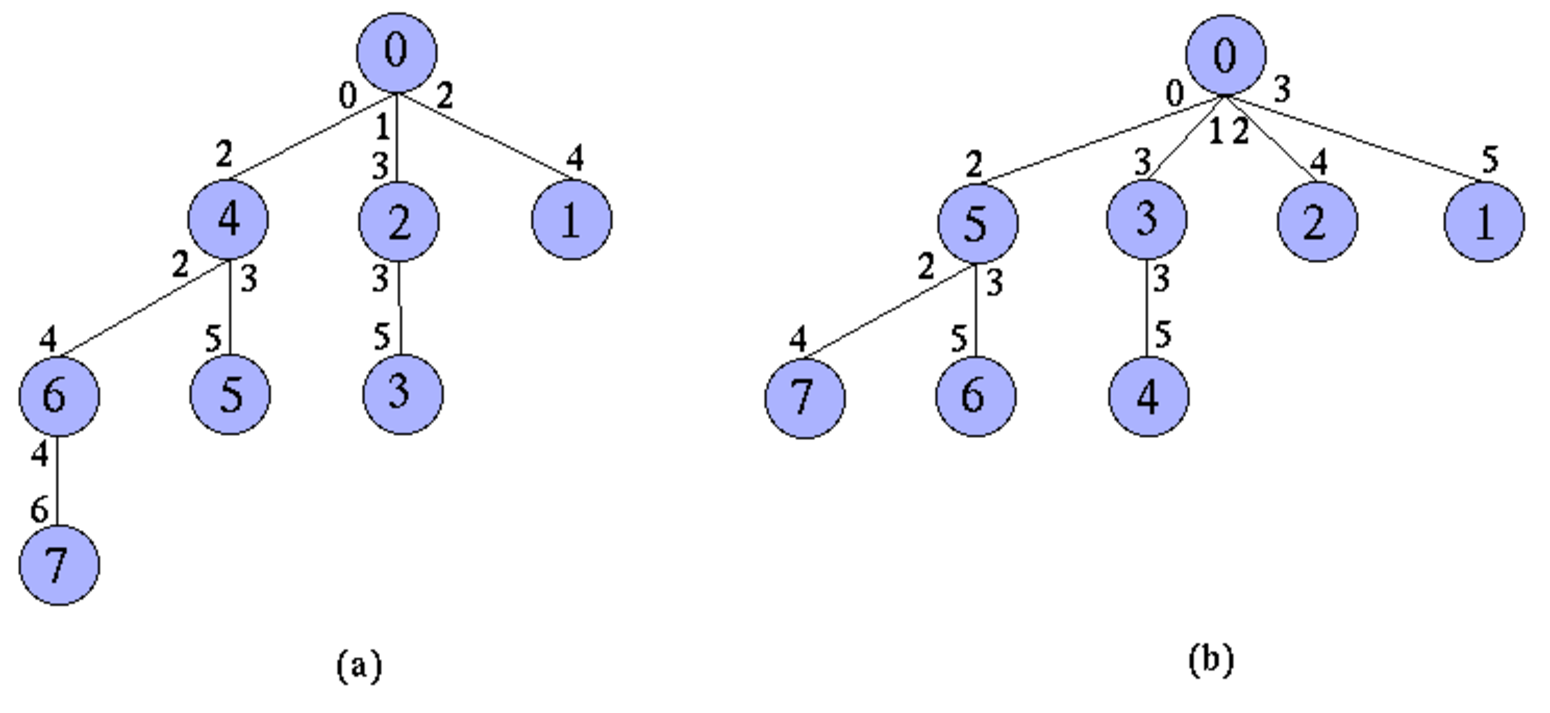
\includegraphics[width=0.85\linewidth]{images/p2p/postal-bcast}
%\par\end{centering}
%
%\caption{\label{Figure:Postal Model}Broadcast avec $\lambda=2$:arbre binomial
%et arbre-$\lambda$}
%
%\end{figure}
%


\subsection{Modélisation des Communications}

Malgré le développement de processeurs et de réseaux plus efficaces,
la communication efficace entre ces deux éléments a toujours été un
obstacle à l'obtention de meilleures performances. En effet, l'augmentation
du nombre de processeurs ne permet pas nécessairement que le temps
d'une application soit réduit proportionnellement : en dehors des
limitations dues au grain des tâches, le coût de communication entre
les différents processeurs est l'un des plus importants obstacles.

Le modèle de Hockney \cite{Hockney94} est un des plus utilisés pour
décrire la communication point-à-point dans les machines parallèles
à mémoire distribuée. Selon ce modèle, une communication entre deux
noeuds est décrite par : 

\[
t=t_{0}+\frac{m}{r_{\infty}}\]


où $t_{0}$ représente le temps nécessaire à l'envoi d'un message
de taille zéro, \emph{m} est la taille du message (en octets) et $r_{\infty}$
est le débit asymptotique en Moctets/s, i.e., le débit maximal obtenu
quand la taille du message s'approche de l'infini. Dans ce raisonnement,
$m/r_{\infty}$ représente le délai de transmission d'un message de
\emph{m} octets à travers un réseau avec un débit asymptotique de
$r_{\infty}$ Moctets/s.

Ce modèle est souvent transformé dans l'équation affine 

\[
t=\alpha+\beta m\]


où $\alpha$ correspond à la latence de transmission et $\beta$ est
le temps de transfert d'un octet sur ce réseau \cite{Pjesivac-Grbovic05}.
L'obtention des paramètres $\alpha$ et $\beta$ peut se faire à travers
l'utilisation de certains outils comme NWS \cite{Wolski97}. 

Toutefois, un inconvénient de ce modèle est qu'il assume que le temps
de transfert est proportionnel à la taille du message. Dans des situations
réelles, certains facteurs comme la taille de la mémoire tampon et
la segmentation des messages en paquets font varier le temps de transfert
$\beta$ selon la taille du message. 

À partir de l'observation qu'un des principaux paramètres pour la
modélisation des algorithmes parallèles est le coût de communication
entre les processus, Bar-Noy et Kipnis ont proposé le modèle Postal
\cite{Bar-Noy94}. Le modèle Postal est fondé sur un paramètre $\lambda=t_{u}/t_{snd}$,
où $t_{snd}$ est le temps nécessaire à un processus pour envoyer
un message (la latence d'envoi), alors que $t_{u}$ représente le
temps total nécessaire à la réception du message par le processus
destinataire. Une des innovations du modèle Postal par rapport à ses
prédécesseurs est que ce modèle permet des situations où un processus
peut émettre plusieurs messages avant que le premier récepteur a reçu
son message : cela est dû à une analogie avec l'envoi de lettres par
la poste. 

%Ces deux modèles pêchent toutefois par le fait qu'ils considèrent un coût de transmission linéaire par rapport aux tailles des messages, ce qui n'est pas exact. 
%
Dans une tentative de spécifier un modèle de calcul plus réaliste,
Culler \emph{et al.} \cite{Culler96} ont proposé le modèle de coût
LogP afin de permettre la spécification du surcoût d'envoi, qui
est normalement très significatif pour la performance d'un système.
L'importance de ce paramètre est notamment observée sur des expériences
en machines réelles et, surtout, dans le cas des clusters (clusters d'ordinateurs). 

%Une autre caractéristique du modèle LogP est son comportement asynchrone. En effet, le modèle LogP ne
%requiert ni barrière de synchronisation, ni super-pas. Quand un processus
%finit l'exécution d'un groupe de tâches et de communications, il peut
%automatiquement avancer vers le prochain groupe de tâches, même s'ils
%existent encore des processeurs travaillant sur une tâche précédente.
%En contraste, le modèle BSP forçait le processeur à rester à l'attente
%de la barrière de synchronisation. Ainsi, ce comportement asynchrone
%du modèle LogP peut être considéré comme un avantage, notamment si
%l'application permet l'avancement asynchrone des différentes lignes
%d'exécution. 

Bien sûr, LogP reste un modèle simplifié des architectures parallèles,
dont certains aspects de la topologie du réseau, comme par exemple
la congestion, ne sont pas directement considérés. Les paramètres LogP qui caractérisent
la communication entre les processus sont les suivants : 

\begin{description}
\item [{L}] - représente la latence de communication entre deux processus
distincts,
\item [{o}] - le surcoût d'initialisation associée à l'envoi/réception
d'un message,
\item [{g}] - aussi appellé "\textit{gap}", cette valeur correspond au temps minimal nécessaire entre deux événements consécutifs
d'envoi ou de réception,
\item [{P}] - le nombre de processus.
\end{description}
Sous cette représentation, le modèle Postal de Bar-Noy et Kipnis devient
un cas spécial du modèle LogP (avec $g=1$ et $o=0$). 

Dans le cas du modèle LogP, le nombre maximum de messages en transit
entre deux processus est de $\lceil L/g\rceil$. La latence maximale
d'un réseau est la distance moyenne asymptotique entre les processus
; toutefois, dans le cas des réseaux fortement hétérogènes, la définition
de ces limites est bien plus complexe. 

%Pour mieux illustrer l'utilisation des paramètres définis par LogP,
%nous présentons dans la Figure \ref{Figure: logp_culler} l'exemple
%proposé par Culler où LogP est utilisé pour décrire le broadcast optimal
%sur un réseau avec $P=8$, $L=6$, $g=4$ et $o=2$. Dans cet exemple,
%nous observons qu'une communication isolée nécessite $o+L+o$ unités
%de temps pour être reçue; cependant, la transmission consécutive de
%deux messages implique un surcoût équivalent à $(g-o)$, car on n'est
%pas autorisé à transmettre deux messages consécutives en moins de
%$g$ unités de temps. En effet, le temps $o$ correspond au temps
%nécessaire au traitement du message pour la transmission (encapsulation,
%mise en mémoire tampon, etc.), alors que le gap $g$ correspond à
%l'intervalle où le réseau reste occupé par la transmission du message.
%
%%
%\begin{figure}[h]
%\begin{centering}
%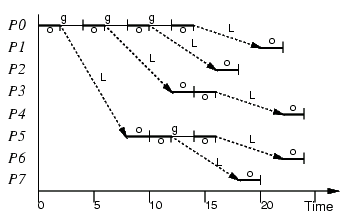
\includegraphics[width=0.6\linewidth]{images/p2p/LogP-optimal}
%\par\end{centering}
%
%\caption{\label{Figure: logp_culler}Diffusion en LogP avec P=8, L=6, g=4 et
%0=2 \cite{Culler96}}
%
%\end{figure}
%


%\subsection{LogGP}
%
%Comme le comportement asynchrone de plusieurs machines parallèles
%et le surcoût de communication sont représentés par le modèle LogP,
%ce modèle est bien plus complet que les modèles précédents. Cependant,
%la faiblesse de ce modèle est que ses paramètres sont établis de façon
%absolue : les valeurs de \emph{g} et \emph{o} sont les mêmes pour
%n'importe quelle taille de message envoyé. Des expériences pratiques
%démontrent que l'utilisation de LogP n'est précise que pour des messages
%de petite taille, dont \emph{g} et \emph{o} ne varient pas trop.
%
%Pour permettre l'utilisation du modèle LogP avec des messages plus
%grands, Alexandrov \emph{et al.} \cite{Alexandrov95} ont présenté
%LogGP, une extension du modèle LogP qui établit le paramètre \emph{G},
%qui représente une valeur de \emph{gap} par octet transmis. À travers
%ce nouveau paramètre, LogGP permet la prédiction du temps de transmission
%d'un message de taille \emph{m} entre deux noeuds avec l'expression
%:
%
%\[
%L+2\times o+(m-1)\times G\]
%
%

\subsection*{pLogP}

Le modèle pLogP (\emph{parameterised LogP}) est une extension
du modèle LogP présenté par Kielmann \emph{et al.} \cite{Kielmann01}. Son objectif est de 
mieux représenter à la fois des petits et des grands messages sous un modèle unifié. 

Comme ses prédécesseurs, le modèle pLogP est défini à travers des
paramètres qui représentent la latence, les surcoûts d'initialisation,
le \emph{gap} et le nombre de processus. La première différence est
l'utilisation de valeurs distinctes, $o_{r}$ et $o_{s}$, pour représenter
le surcoût d'envoi et le surcoût de réception d'un message. Toutefois,
la principale caractéristique du modèle pLogP est que les paramètres
qui représentent le \emph{gap} et les surcoûts sont paramétrés selon
la taille du message envoyé. Cela est spécialement important pour
modéliser les communications avec des tailles de messages variables,
une fois que, comme déjà observé par Alexandrov \cite{Alexandrov95},
la performance des communications n'est pas linéaire par rapport à
la taille des messages.

D'autres aspects sont aussi différents, par rapport aux modèles précédents.
En effet, les notions de la latence et du \emph{gap} sont légèrement
différentes de celles utilisées par le modèle LogP. Dans le
cas du modèle pLogP, la latence inclut tous les facteurs qui peuvent
retarder la communication entre deux processus, comme par exemple
la copie de données en mémoire tampon vers les interfaces réseaux,
qui s'ajoutent au temps de transfert des messages déjà considéré par
LogP. Ainsi, dans le cas d'un réseau local, le paramètre \emph{gap}
est défini comme l'intervalle minimale entre deux transmissions ou
réceptions consécutives, ce qui implique que $g(m)\geq os(m)$ et
$g(m)\geq or(m)$ tient toujours. La relation entre ces différents
paramètres est illustrée dans la Figure \ref{Figure: pLogP}. 

%
\begin{figure}[h]
\centering
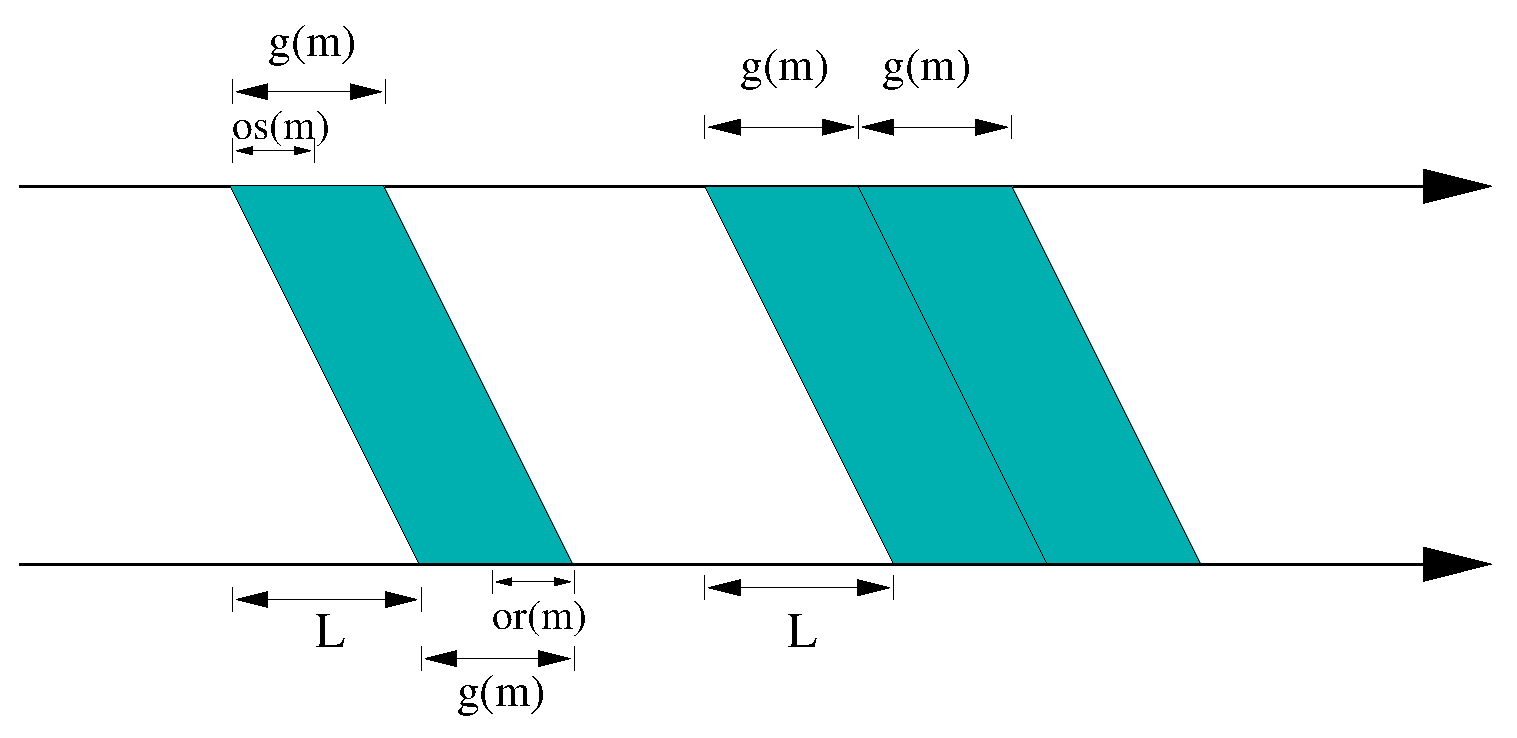
\includegraphics[width=0.7\linewidth]{images/p2p/plogp-struct}

\caption{\label{Figure: pLogP}Représentation d'une communication avec pLogP}

\end{figure}


En conséquence de cette nouvelle interprétation du \emph{gap}, les
paramètres $o_{s}$ et $o_{r}$ ont une importance moins évidente,
une fois que leur coût dans un réseau local est souvent recouvert
par celui du gap.  Ainsi, pour représenter le temps nécessaire à la transmission d'un
message de taille \emph{m} entre deux n{\oe}uds avec des primitives de
communication bloquante, le modèle pLogP utilise l'expression $L+g(m)$,
au lieu de $L+g+2o$ comme dans le modèle LogP. 


La variation des paramètres vis-à-vis de la taille des messages et des politiques d'émission est mise en évidence en Figure \ref{Figure: logp x hockney}, où on affiche les différents temps de communication mesurés avec la bibliothèque applicative LAM-MPI \cite{LAM04}. On observe un
changement de politique d'acquittement quand la taille des messages dépasse les 64 Ko, de manière à ce que le coût du gap dépend à la fois
de la saturation de la fenêtre TCP et de la politique d'acquittement.

%
\begin{figure}
\centering
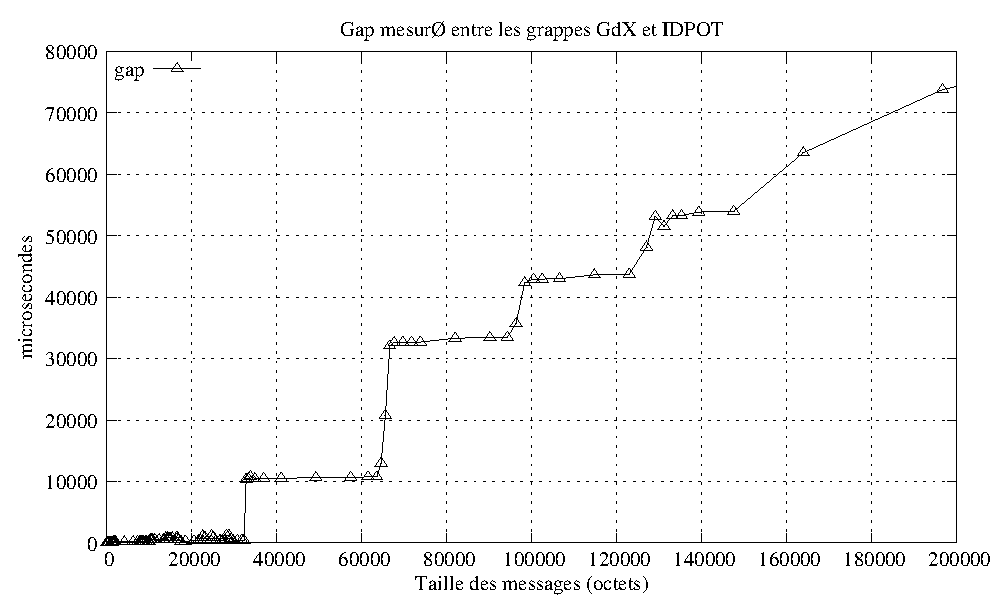
\includegraphics[width=0.7\linewidth]{images/p2p/hockney-logp1}

\caption{\label{Figure: logp x hockney}Valeurs de gap mesurés entre deux machines
distantes}

\end{figure}



\section{Modélisation de l'Opération de Diffusion Broadcast}

Parmi les opérations de communication collective, les diffusions de type Broadcast sont parmi les plus simples et les plus répandues. Une opération de \emph{Broadcast} s'effectue quand un seul processus,
appelé \emph{racine,} envoie le même message de taille \emph{m} à
tous les autres $(P-1)$ processus.  Ceci représente en effet le patron de communication \textit{one-to-all}. 

Dans le cas du calcul distribué, la diffusion d'opérations est souvent nécessaire afin d'apporter des paramètres et données à tous les n{\oe}uds.  La compréhension de ses mécanismes et la modélisation de ses coûts présente un intérêt stratégique vis-à-vis de la scalabilité et l'optimisation des algorithmes. Dans ce sens, il est aussi nécessaire prendre en compte les différences architecturales des environnements de communication : les stratégies efficaces pour un environnement homogène diffèrent de celles adaptées aux environnements hétérogènes. Afin de représenter ces deux cas, nous nous sommes intéressés à la modélisation et optimisation des communications collectives de type Broadcast dans deux types distincts de réseaux : les clusters (grappes de machines) et les grids (grilles de calcul). Le premier cas souvent peut être considéré comme homogène, alors que le deuxième apporte un degré d'hétérogénéité à cause des différences de communication intra et inter-cluster. Afin d'implémenter et valider ces stratégies, nous avons choisi d'utiliser comme point de départ la bibliothèque de passage de messages MPI (Message Passing Interface), très utilisée par la communauté du calcul parallèle et qui dispose déjà d'une implémentation simple de l'opération broadcast appelée MPI\_BCast.   

\subsection{\label{sec:Broadcast}Modélisation d'un Broadcast dans un réseaux homogène}

L'opération \emph{Broadcast} est une des plus simples opérations de
communication collective : initialement, seul le processus \emph{racine}
détient le message qui doit être diffusé ; à la fin de l'opération,
une copie de ce message est déposée dans chaque processus du groupe.
L'approche classique pour implémenter l'opération \emph{Broadcast} utilise
des arbres qui sont décrits par deux paramètres, \emph{d} et \emph{h},
où \emph{d} est le nombre maximum de successeurs qu'un n{\oe}ud peut
avoir, et \emph{h} est la hauteur de cet arbre, le chemin le plus
long qui relie la racine et les feuilles de cet arbre. Plus généralement,
des arbres de diffusion avec différents degrés \emph{d} et \emph{h}
peuvent être générés à partir d'un algorithme de type \emph{arbre-alpha}
(\emph{alpha-tree} en anglais) suggéré par Bernaschi et Ianello \cite{Bernaschi98}.
À l'aide de cet algorithme et des paramètres du réseau, un arbre optimal
peut être construit à partir des paramètres du réseau et avec \emph{d,
	h $\in$}{[}1...\emph{P}-1] tel que $\sum_{i=o}^{h}d^{i}\geq P$ soit
respecté. %Cependant, pour une question de simplicité, la plupart des
%implémentations MPI utilisent des formes fixes telles que les arbres
%plats ou les arbres binomiaux. 

La performance des différentes formes fixes dépend surtout des paramètres
du réseau, notamment le \emph{gap}, la latence et le nombre de n{\oe}uds.
Par conséquent, un réseau avec une latence faible par rapport au \emph{gap}
favorise les algorithmes de type Arbre Binaire et Arbre Binomial,
qui cherchent à minimiser le temps de communication par la multiplication
des sources de transmission. Au contraire, si la latence est trop
élevée par rapport au \emph{gap}, les algorithmes de type Arbre Plat
sont favorisés, où un seul processus envoie des messages à tous les
autres. 


À partir des modèles de coût LogP \cite{Culler96} et pLogP \cite{Kielmann01}
et de travaux comme ceux de Huse \cite{Huse99}, Vadhiyar \cite{Vadhiyar00}
et autres, nous avons déduit les formules qui représentent différentes
stratégies de communication évaluées dans ce travail, comme indiqué
dans le Tableau \ref{table:bcast_models_classique}. Certaines de
ces stratégies sont clairement inefficaces, comme par exemple le broadcast
en Chaîne, qui exécute $P-1$ communications en série. 

%
\begin{table}
	\centering
	\begin{tabular}{|c|c|}
		\hline 
		\textbf{\small Stratégie} & \textbf{\small Modèle de Communication}\tabularnewline
		\hline
		\hline 
		{\small Arbre Plat} & {\small $L+(P-1)\times g(m)$}\tabularnewline
		\hline 
		{\small Arbre Plat Rendez-vous} & {\small $3\times L+(P-1)\times g(m)+2\times g(1)$}\tabularnewline
		\hline 
		{\small Chaîne} & {\small $(P-1)\times(g(m)+L)$}\tabularnewline
		\hline 
		{\small Arbre Binaire} & {\small $\leq\lceil log_{2}P\rceil\times(2\times g(m)+L)$}\tabularnewline
		\hline 
		{\small Arbre Binomial} & {\small $\lceil log_{2}P\rceil\times L+\lfloor log_{2}P\rfloor\times g(m)$}\tabularnewline
		\hline
	\end{tabular}
	
	
	\caption{\label{table:bcast_models_classique}Modèles de communication pour
		le \emph{Broadcast}}
	
\end{table}

%\subsubsection{\label{sub: approches par segmentation}Approches par segmentation}

Une autre possibilité de construire un \emph{Broadcast} est la composition
des chaînes de retransmission \cite{Barnett96}. Cette stratégie,
possible grâce à la segmentation des messages, présente des avantages
importants, comme l'indiquent \cite{Kielmann01}\cite{Thakur03}\cite{Beaumont04a}.
Dans un \emph{Broadcast} Segmentée, la transmission des messages en
segments permet le recouvrement de la transmission d'un segment \emph{k}
et la réception du segment \emph{k}+1, minimisant le \emph{gap}.

Dans ce cas, nous considérons que le segment de taille \emph{s} d'un
message \emph{m} est un multiple de la taille du type basique de données
qui est transmis, divisant alors le message initial \emph{m} en \emph{k}
segments. Par conséquent, \emph{g(s)} représente le \emph{gap} d'un
segment de taille \emph{s}. Toutefois, le choix de la taille des segments
reste dépendant des caractéristiques du réseau. En effet, l'utilisation
de segments trop petits a un surcoût non-négligeable dû à l'en-tête
du message, alors que l'utilisation des segments trop grands ne permet
pas l'exploitation intégrale du débit du réseau. 

La recherche de la taille de segment \emph{s} qui minimise le temps
de communication se fait à l'aide des modèles de communication présentés
dans le Tableau \ref{table:bcast_models_seg}. D'abord, on cherche
une taille de segment \emph{s} qui minimise le temps de communication
parmi $s=m/2^{i}\;\mathrm{pour}\; i\in[0\ldots log_{2}m]$. Ensuite,
on peut affiner la recherche de la taille optimale avec l'aide d'heuristiques
comme le \emph{\og local hill-climbing} \fg{} \cite{Kielmann01}.

%
\begin{table}
	\centering
	\begin{tabular}{|c|c|}
		\hline 
		\textbf{\small Stratégie} & \textbf{\small Modèle de Communication}\tabularnewline
		\hline
		\hline 
		{\small Arbre Plat Segmenté} & {\small $L+(P-1)\times(g(s)\times k)$}\tabularnewline
		\hline 
		{\small Chaîne Segmentée (Pipeline)} & {\small $(P-1)\times(g(s)+L)+(g(s)\times(k-1))$}\tabularnewline
		\hline 
		{\small Arbre Binomial Segmenté} & {\small $\lceil log_{2}P\rceil\times L+\lfloor log_{2}P\rfloor\times g(s)\times k$}\tabularnewline
		\hline
		{\small Pieuvre avec un degré }\emph{\small d} & {\small $(d+\lceil\frac{P-(2^{d}+1)}{(2^{d}+1)}\rceil)\times(g(s)+L)+(g(s)\times(k-1))$}\tabularnewline
		\hline
		{\small Scatter/Collection \cite{Thakur03}} & {\small $(log_{2}P+P-1)\times L+2\times(\frac{p-1}{p})\times g(m)$}\tabularnewline
		\hline
	\end{tabular}
	
	\caption{\label{table:bcast_models_seg}Modèles de communication segmentée
		pour le \emph{Broadcast}}
	
\end{table}


Pour valider ces modèles de communication, nous avons choisi la comparaison
entre les prédictions des modèles et les résultats réels obtenus à
partir d'expérimentations sur différentes plates-formes réseaux. Pour
illustrer notre approche, nous avons comparé des implémentations de
MPI\_Bcast selon les stratégies Arbre Plat, Arbre Binomial et Chaîne
Segmentée. Ainsi, les Figures \ref{Figure:Comparison-Bcast_Flat_FEth}
et \ref{Figure:Comparison-Bcast-Chain_FEth},
illustrent les valeurs mésurées expérimentalement des trois stratégies d'implémentation, qui suivent presque
fidèlement les prédictions des modèles.
%Dans les prochaines pages nous présentons l'analyse des
%expérimentations effectuées sur chaque plate-forme réseau différente. 


%le réseau Fast Ethernet. 
\begin{figure}[h]
	\centering
	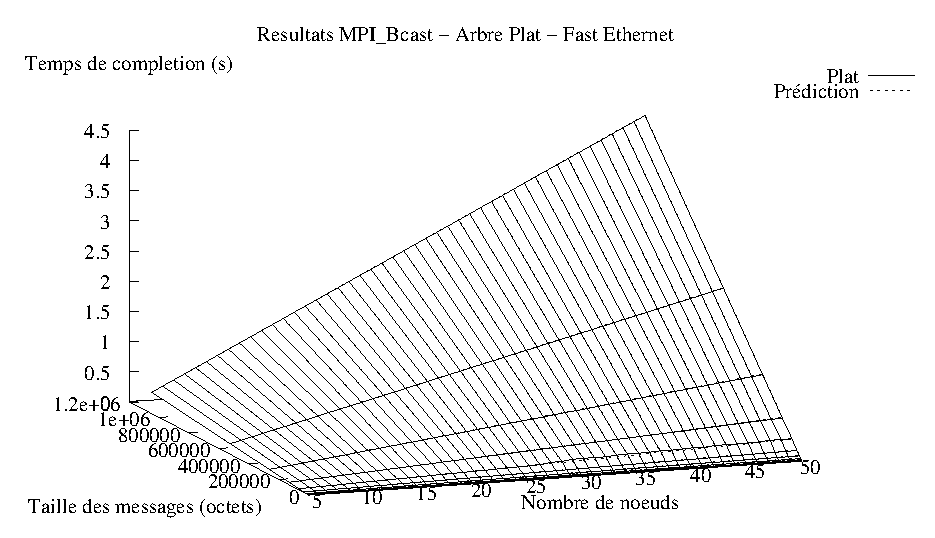
\includegraphics[width=0.5\linewidth]{images/modeles/FEth/Bcast/comp_Flat}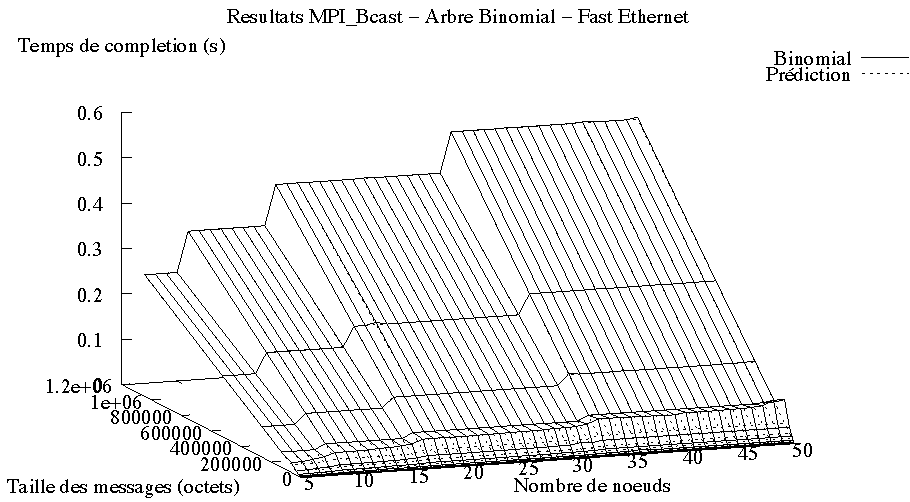
\includegraphics[width=0.5\linewidth]{images/modeles/FEth/Bcast/comp_Binomial}
	\caption{\label{Figure:Comparison-Bcast_Flat_FEth}Les performances réelles
		et prédites pour l'Arbre Plat (a) et l'Arbre Binomial (b) avec un réseau Fast Ethernet}
\end{figure}

%
\begin{figure}[h]
	\centering
	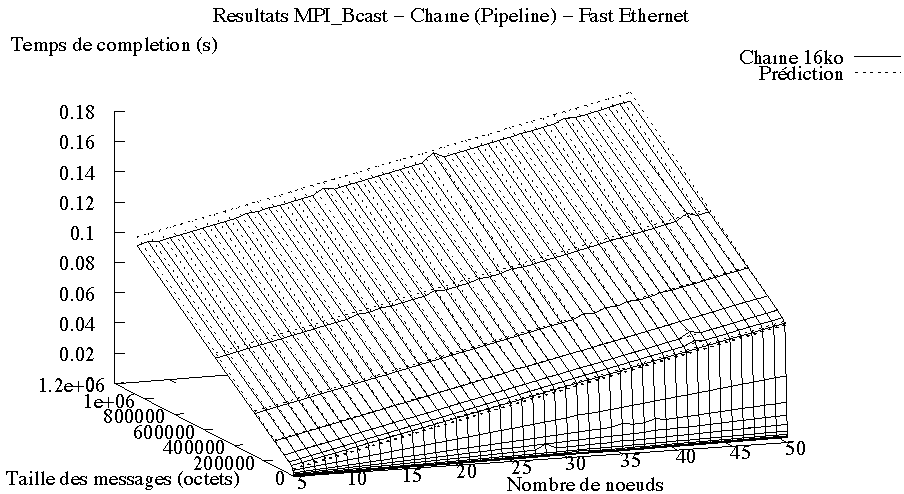
\includegraphics[width=0.5\linewidth]{images/modeles/FEth/Bcast/comp_Chain_16384}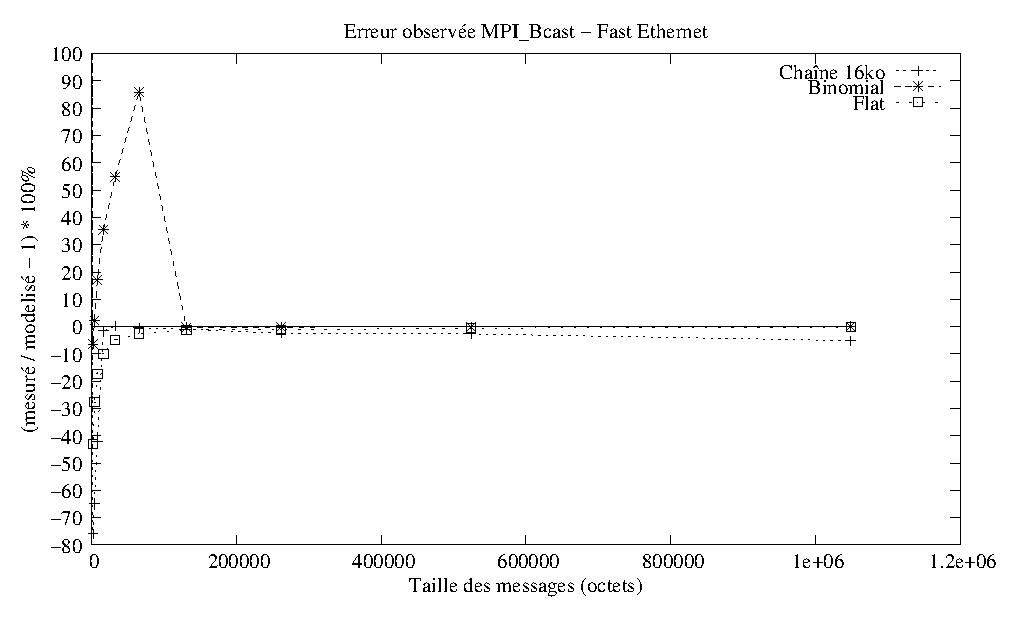
\includegraphics[width=0.5\linewidth]{images/modeles/FEth/Bcast/error}
	\caption{\label{Figure:Comparison-Bcast-Chain_FEth}Performances réelles
		et prédites pour la Chaîne Segmentée (a)  et l'erreur des prédictions par rapport
		aux valeurs mesurées (b)}
\end{figure}

Plus spécifiquement, des différences entre les prédictions et les
valeurs réelles sont observées surtout dans le cas de l'envoi de petits messages, qui ne suit pas un comportement linéaire
par rapport à la taille des messages. Cette variation de performance
a été l'objet d'analyses précédentes (cette discussion peut être retrouvée
dans les articles \cite{Steffenel04a} et \cite{Steffenel04c}) et doit son origine à l'implémentation des politiques de 
transmission et d'acquittement TCP, qui parfois opte pour retarder l'envoi de petits messages. 

En effet, TCP dispose d'une option \emph{socket} TCP\_NODELAY qui devrait permettre l'envoi de tout message sans attente. 
Seulement, nous avons observé que parfois un seul message
à chaque \emph{n} messages transmis n'est pas acquitté comme il le
faut. Cette défaillance de l'implémentation protocole d'acquittement induit un temps supplémentaire
 qui se reflète sur un surcoût lors de l'envoi de petits messages.  


La Figure \ref{Figure:Comparison-Bcast-Chain_FEth} résume aussi ces trois stratégies en affichant le taux d'erreur entre les mesures et les prédictions.
Ici, nous observons que les résultats réels, normalement très proches
des prédictions (à une marge de 10\% maximum), s'écartent des prédictions
jusqu'à 90\% pour des messages autour de 128 Ko. Néanmoins, ces variations
affectent des communications où la différence absolue n'est que de
quelques millisecondes, ce qui n'empêche pas l'utilisation des modèles
de communication pour choisir la meilleure stratégie de communication. 


\subsection{Modélisation du Broadcast dans un Grid}

La détermination du meilleur arbre de diffusion pour un environnement
homogène est une tâche relativement facile car dépend de paramètres de latence et débit (gap) communs à tout le réseau.  

Cependant, dans le cas d'un réseau hétérogène, ce problème devient
bien plus difficile à cause des variations des paramètres de communication entre chaque pair de n{\oe}uds. En effet, l'identification du meilleur arbre
de diffusion dans un réseau hétérogène est un problème NP-complet \cite{Bhat99}\cite{Beaumont04c,Beaumont05b}\cite{PangfengLiu04}.
La plupart des travaux dédiés à l'optimisation des communications
collectives dans des environnements hétérogènes essayent donc de construire des arbres de diffusion en tenant compte du coût d'interconnexion entre chaque pair de processus concernée par le broadcast. C'est le cas de Banikazemi \cite{Banikazemi98},
Bhat \cite{Bhat99,Bhat03} ou Mateescu \cite{Mateescu05}.

Cependant, l'environnement de type grid est normalement caractérisé
par un grand nombre de processus communicants, résultat de l'association
des différentes clusters. Dans ce cas, la complexité de la
tâche d'optimisation est bien plus importante, et des simplifications
s'imposent afin de permettre l'utilisation de telles méthodes dans
la pratique. Une de ces simplifications est le regroupement des processus
selon leurs performances relatives (par exemple, par rapport à la
communication), de manière à ce que toute une classe de processus
puisse être traitée comme une entité unique. De cette manière, le nombre important de processus dans un grid peut être
encore facilement abordable par les méthodes d'optimisation classiques grâce à la division des communications en deux catégories, l'\textit{inter-cluster} et l'\textit{intra-cluster}. 


Cependant, à défaut de leur apport aux algorithmes de Broadcast, ces
techniques peuvent encore être améliorées. En effet, les travaux précédents
ont été établis dans un contexte où les communications de longue distance
étaient plusieurs ordres plus lentes que celles à l'intérieur des
réseaux locaux, et la réduction des communications inter-clusters permettait
la minimisation de la congestion sur les liens les plus lents. Si
cela est encore vrai en ce qui concerne la latence entre les n{\oe}uds,
il n'est plus exact pour le débit d'un lien de longue distance. D'autre
part, le faible coût du matériel informatique permet aujourd'hui que
les  clusters regroupent des centaines de n{\oe}uds. Or, plus le coût de
diffusion \og intra- clusters \fg{} devient important, plus son influence
sur la performance sera importante au moment de définir l'ordonnancement
des communications.

C'est exactement ce qui différencie les heuristiques traitant (ou
ne traitant pas) la communication à l'intérieur des groupes : les
heuristiques \og traditionnelles \fg{} et celle appelées \og heuristiques
sensibles au contexte des grids \fg{} (\og \emph{grid-aware} \fg{}
en anglais). Dans le premier cas, l'optimisation ne tient compte que
des communications entre les différents coordinateurs, alors que le
deuxième cas s'occupe aussi de la diffusion à l'intérieur des  clusters. 


Les prochaines sections présentent les différentes heuristiques étudiées
pour l'optimisation des communications de type MPI\_Bcast. Certaines
de ces heuristiques sont la simple application des méthodes pour les
réseaux hétérogènes dans le contexte des  clusters hiérarchisées. Dans
ce travail nous proposons trois nouvelles méthodes, qui au contraire
des techniques précédentes, considèrent autant les communications
entre les coordinateurs que les temps nécessaires à la diffusion des
messages à l'intérieur des  clusters.


\subsubsection*{Formalisme utilisé}

Pour décrire les heuristiques présentées dans cette section, nous
utilisons un formalisme de groupes similaire à celui de Bhat \cite{Bhat03}.
Dans ce formalisme, les  clusters sont séparées en deux groupes, \textbf{A}
et \textbf{B}. Le groupe \textbf{A} contient les  clusters qui ont déjà
reçu le message (la réception du message par le coordinateur du
 cluster est suffisante). Le groupe \textbf{B} contient les  clusters
qui devront recevoir le message. De cette manière, le groupe \textbf{A}
contient initialement le  cluster du processus \emph{source} ou \emph{racine},
tandis que le groupe \textbf{B} contient toutes les autres  clusters
du réseau.

À chaque étape, un émetteur appartenant au groupe \textbf{A} et un
récepteur appartenant au groupe \textbf{B} sont choisis. Après la
communication entre ces deux  clusters (plus exactement, leurs coordinateurs),
le cluster récepteur est transféré au groupe \textbf{A}. 

L'implémentation de ces communications est faite de manière à rendre
prioritaires les communications entre les  clusters. En effet, les coordinateurs
diffusent le message à l'intérieur de ses  clusters seulement après
la fin des communications inter- clusters. Cette stratégie favorise
la multiplication des sources disponibles et l'application des heuristiques,
ainsi que la prédiction du temps total d'exécution du Broadcast.

\subsubsection{Heuristiques Traditionnelles}

\subsubsection*{Diffusion en Arbre Plat (Flat)}

L'heuristique en \emph{Arbre Plat}, découpe la communication en deux niveaux, \emph{inter- clusters}
et \emph{intra- clusters}. 

Dans le premier niveau, le processus \emph{racine} envoie le message
à tous les coordinateurs des différentes  clusters. L'ordre d'envoi
suit le \og rang \fg{} des différentes  clusters, prédéfini à l'initialisation.
Formellement, cela veut dire qu'à chaque étape, le processus \emph{racine}
choisi comme récepteur le premier  cluster du groupe \textbf{B}. Dans
cette \og heuristique \fg{}, le processus émetteur est toujours
le même (le processus \emph{racine}), malgré le fait que les  clusters
qui ont déjà reçu le message font désormais partie du groupe \textbf{A}.
Dans le deuxième niveau de diffusion, exécuté à l'intérieur de chaque
 cluster, les coordinateurs exécutent un \emph{broadcast} en arbre binomial.

Même si cette heuristique est très simple à implémenter, elle est toutefois
très peu optimisée. En effet, la diffusion des données ne tient pas
compte des performances des différents  clusters, ni les vitesses d'interconnexion
entre les \emph{coordinateurs}. Même si l'utilisateur organise le
fichier de description des  clusters de manière à favoriser les communications
émises d'un certain  cluster, celles-ci restent soumises à une structure
de diffusion \emph{plate}. 


\subsubsection*{Fastest Node First - FNF}

L'heuristique \emph{Fastest Node First} (le n{\oe}ud le plus rapide d'abord)
a été proposée par Banikazemi \emph{et al.} \cite{Banikazemi98}.
Dans leur modèle de communication, le réseau est composé d'un certain
nombre de n{\oe}uds \emph{$P$}. À chaque n{\oe}ud \emph{$P_{\textrm{i}}$}
on associe un coût d'envoi \emph{$C_{\textrm{i}}$}. Ce coût \emph{$C_{\textrm{i}}$}
est indépendant de la destination et de la taille du message, et indique
seulement la différence de vitesse entre les n{\oe}uds.

L'heuristique proposée par Banikazemi \emph{et al.} nécessite $P-1$
itérations, où à chaque étape l'heuristique définie un émetteur et
un récepteur. Le récepteur est choisi parmi les possibles récepteurs
du groupe \textbf{B} dont le coût \emph{$C_{\textrm{i}}$} est le
plus petit. L'émetteur est le processus du groupe \textbf{A} qui peut
finir la communication le plus rapidement possible. Cela dit, cette
stratégie choisit l'émetteur le plus rapide et le récepteur qui pourrait
retransmettre les messages le plus rapidement possible, à son tour.

L'efficacité de l'heuristique FNF dans le cadre des environnements
homogènes a été démontrée par Liu \cite{PangfengLiu00b}, qui a prouvé que
l'heuristique FNF produit des ordonnancements avec au plus deux fois
le temps optimal.

Cependant, des environnements homogènes comme ceux considérés par
Banikazemi sont assez rares dans les grids, ce qui rend cette heuristique
très limitée par rapport à la modélisation des communications. En
effet, le modèle de coût unique $C_{\textrm{i}}$ n'est pas suffisant
pour représenter l'hétérogénéité d'un réseau d'interconnexion, comme
indiqué par Bhat \cite{Bhat03}. 


\subsubsection*{Fastest Edge First - FEF}

Proposée par Bhat \emph{et al.} \cite{Bhat03}, l'heuristique \emph{Fastest
	Edge First} (l'arête la plus rapide d'abord) est un algorithme glouton
qui fait partie d'une collection d'heuristiques proposées comme alternative
à l'heuristique FNF. 

Assez simple, cette heuristique est très similaire à l'heuristique
FNF. Seulement, au lieu d'un coût de communication unique $C_{\textrm{i}}$,
l'heuristique évalue le poids de chaque lien de communication $L_{i,j}$
entre deux n{\oe}uds différents (les arêtes), correspondants à la latence
de communication entre les deux processus. 

Pour identifier l'ordonnancement des communications nécessaire à l'exécution
de l'opération de Broadcast, l'algorithme FEF, ordonne les processus
du groupe A selon leurs arêtes les plus rapides. Cela permet le choix
du lien le plus rapide parmi toutes les possibilités, et en même temps,
sert à définir l'émetteur et le récepteur, déterminés implicitement
par l'arête choisie. Une fois que le récepteur est désigné, celui-ci
est transféré du groupe \textbf{B} vers le groupe \textbf{A}. À cet
instant, les arêtes minimales doivent être recalculées.

Le raisonnement de cette heuristique est que le choix des liens les
plus rapides permet d'augmenter rapidement le nombre d'émetteurs.
À leur tour, ces émetteurs pourront disséminer le message vers les
processus les plus éloignés, tout en choisissant le lien le moins
coûteux.


\subsubsection*{Early Completion Edge First - ECEF}

Selon les heuristiques précédentes, une fois que le récepteur était
assigné, celui-ci était immédiatement transféré vers le groupe des
émetteurs, le groupe \textbf{A}. Toutefois, à cause des délais de
communication, il est possible que ce récepteur n'ait pas encore reçu
le message et qu'il soit choisi pour le retransmettre à un deuxième
processus. La communication subira un retard supplémentaire, alors
qu'une autre arête, moins rapide, pourrait finir la transmission plus
vite si son émetteur a déjà le message. 

Pour tenir compte des retards dus à la transmission des données, l'heuristique
\emph{Early Completion Edge First} (arête qui finit le plus tôt) considère
aussi dans son évaluation l'instant où les émetteurs ont les données
disponibles pour l'envoi. Ainsi, la \emph{disponibilité} $RT_{i}$
du processus émetteur (\emph{Ready Time} en anglais) est alors utilisée
conjointement avec le temps nécessaire à la transmission du message
entre les processus (le gap plus la latence) de manière à choisir
le couple émetteur-récepteur qui minimise le temps : 

\[
RT_{i}+g_{i,j}(m)+L_{i,j}\]


Ainsi, l'objectif de cette heuristique est d'augmenter le nombre de
processus qui peuvent \emph{effectivement} transmettre les messages
aux autres processus.


\subsubsection*{Early Completion Edge First with lookahead - ECEF-LA}

Pour augmenter l'efficacité de l'heuristique précédente, la dernière
heuristique proposée par Bhat \emph{et al.} \cite{Bhat03} propose
une recherche plus approfondie sur les possibles choix. En effet,
si l'objectif des heuristiques précédentes était la multiplication
des sources disponibles, cela suppose que ces sources pourront, à
leur tour, retransmettre les messages de manière efficace.

C'est ainsi que Bhat a proposé l'utilisation d'une fonction de \emph{lookahead}
(recherche en avant) pour évaluer si le choix d'un récepteur est réellement
bon. De cette manière, l'algorithme calcule préalablement la fonction
de \emph{lookahead} $F_{j}$ pour tous les processus dans le groupe
\textbf{B}, et la pair émetteur-récepteur est celle qui minimise
la somme :

\[
RT_{i}+g_{i,j}(m)+L_{i,j}+F_{j}\]


Cette fonction de \emph{lookahead} peut être définie de plusieurs
façons. Bhat \cite{Bhat03} propose, par exemple, le coût minimal
pour que le processus \emph{j} transmette à d'autres processus encore
dans le groupe \textbf{B}. Cette fonction est alors la suivante :

\begin{eqnarray*}
	F_{j} & = & \min_{P_{k}\in B}\,(g_{j,k}(m)+L_{j,k})\end{eqnarray*}


Intuitivement, cette fonction indique l'utilité du processus $P_{j}$
si à son tour il est transféré vers le groupe \textbf{A}. D'ailleurs,
Bhat a proposé d'autres fonctions de \emph{lookahead}, dont par exemple
la moyenne de la latence entre $P_{j}$ et les autres processus en
\textbf{B}, ou alors la latence moyenne entre les émetteurs et les
récepteurs, si on considère que $P_{j}$ est transféré vers le groupe
\textbf{A}. 


\subsubsection{Heuristiques "grid-aware"}

Les heuristiques présentées précédemment hiérarchisent les communications en deux niveaux - \emph{inter- clusters}
et \emph{intra- clusters}, mais les fonctions d'évaluation ne tiennent compte que des coûts de transmission entre les coordinateurs
des différentes  clusters du réseau.

Comme nous l'avons déjà exposé, le coût d'une communication
hiérarchique ne dépend pas seulement des latences entre les différentes
 clusters, mais aussi du temps nécessaire à la diffusion des messages
à l'intérieur de ces  clusters. Ce coût de diffusion intra- clusters devient
encore plus important avec l'augmentation du nombre de n{\oe}uds à l'intérieur
des  clusters, qui aujourd'hui dépasse facilement la centaine de machines.
Par exemple, l'envoi d'un message de 1Mo entre deux clusters (l'un à Grenoble, l'autre à Paris) requiert 349 millisecondes, alors que
le broadcast de ce même message entre 50 n{\oe}uds du cluster de Grenoble
peut nécessiter jusqu'à 3 secondes selon l'algorithme
utilisé. Si ce temps n'est pas pris en compte lors de la modélisation
des communications, l'ordonnancement des communications risque d'être
sous-optimal.

Plus exactement, le temps de diffusion intra- clusters, appelé $T_{k}$,
correspond aux prédictions des modèles de communication vus précédemment. 
Cette notation $T_{k}$ est équivalente à une notation où un n{\oe}ud
fictif $k'$ est associé à chaque coordinateur $k$, dont :

\[
L_{k,k'}+g_{k,k'}=\left\{ \begin{array}{c}
\begin{array}{cc}
T_{k} & si\: k'\, est\, associe\, a\, k\\
\infty & \,\,\,\,\,\,\,\,\,\,\,\,\, pour\, tout\, autre\, processus\, j\neq k\end{array}\end{array}\right.\]


La présence d'un n{\oe}ud fictif permet l'utilisation des heuristiques
précédentes sans la nécessité d'une modification des algorithmes,
notamment le ECEF. L'utilisation de $T_{k}$ permet une implémentation
plus simple des algorithmes, qui n'ont pas besoin de garder les deux
identités \emph{k} et \emph{k'} associées à un  cluster \emph{k}. Toutefois, dans ce travail nous avons gardé
la description séparée \emph{L}, \emph{g} et \emph{T}, afin
de permettre une identification plus facile des facteurs évalués.

Dans ce sens, nous présentons deux nouvelles stratégies d'évaluation
dites \og sensibles au contexte des grids\fg{}, où
le temps de diffusion \emph{intra-cluster} est aussi considéré lors
de la construction des arbres de diffusion. Pour mieux analyser l'efficacité
de ces stratégies, nous avons aussi développé une version de l'heuristique
ECEF-LA où le temps intra- clusters est pris en compte. Cette version
sert de comparaison par rapport aux heuristiques de Bhat, présentées
précédemment. 


\subsubsection*{ECEF-LA\emph{t}}

L'heuristique ECEF-LA\emph{t} est l'évolution naturelle de l'heuristique
ECEF-LA où nous utilisons une fonction de \emph{lookahead} adaptée
à la représentation du coût de communication intra- clusters $T_{k}$. 

Ainsi, l'heuristique ECEF-LA\emph{t} cherche à minimiser le coût total
de transmission et le temps nécessaire à la diffusion d'un message
dans un  cluster distant (en effet, le \og petit \emph{t} \fg{}
du nom de cette heuristique indique qu'on cherche le minimum des temps).
Pour cela, elle utilise une fonction d'évaluation :

\begin{eqnarray*}
	F_{j} & = & \min_{P_{k}\in B}\,(g_{j,k}(m)+L_{j,k}+T_{k})\end{eqnarray*}


À l'instar de l'heuristique ECEF-LA, le but de cette stratégie est
que le récepteur soit choisi parmi les  clusters qui peuvent retransmettre
le message le plus vite possible à d'autres  clusters. L'adjonction
du temps $T_{k}$ dans la fonction d'évaluation implique aussi que
le choix d'un interlocuteur minimisera le temps de complétion des
 clusters contactés dans le futur. 


\subsubsection*{ECEF-LA\emph{T}}

Une contrepartie de la technique précédente est que cette stratégie
a tendance à favoriser les  clusters rapides, ce qui peut entraîner
des retards supplémentaires aux  clusters plus lents, reléguées aux
dernières places. Pour éviter une telle situation, nous proposons
une nouvelle fonction de \emph{lookahead}, où le choix des  clusters
considère le maximum du temps nécessaire à la transmission et à la
diffusion d'un message : 

\begin{eqnarray*}
	F_{j} & = & \max_{P_{k}\in B}\,(g_{j,k}(m)+L_{j,k}+T_{k})\end{eqnarray*}


Malgré sa similarité avec l'heuristique précédente, cette nouvelle
fonction d'évaluation cherche à équilibrer le temps de communication
vers les différents  clusters, lentes ou rapides. En effet, nous cherchons
dans un premier instant le  cluster la plus lente qu'il reste à contacter
(la fonction de \emph{lookahead}), et parmi les choix d'émetteurs
disponibles, nous choisissons celui qui peut la contacter le plus
rapidement possible (fonction d'évaluation \emph{min} de l'heuristique
ECEF).

Le raisonnement de cette heuristique est que si les  clusters les plus
distants ou les plus lents (dans le sens où la diffusion des messages
prend plus de temps) sont contactés en dernière place, leur diffusion
prendra encore plus de retard, ce qui augmentera le temps d'exécution
du Broadcast. Avec la fonction de \emph{lookahead} de ECEF-LA\emph{T},
nous choisissons comme récepteur le  cluster qui prendra le moins de
temps possible pour contacter le  cluster le plus lent : cela garantit
que si besoin est, les  clusters les plus lents seront contactés dans
le minimum de temps possible.


\subsubsection*{BottomUp}

La troisième heuristique proposée dans ce travail utilise une logique
d'optimisation différente de celle utilisée par Bhat. En effet, l'approche
de Bhat vise toujours la minimisation des facteurs liés à la transmission
des messages et à sa diffusion, ce qui généralement finit par donner
priorité aux  clusters les plus rapides. Cependant, nous considérons
que le temps d'exécution d'un Broadcast hiérarchique dépend surtout
des  clusters les plus lents.

À partir des heuristiques précédentes, nous observons que, malgré
l'utilisation de différentes fonctions de \emph{lookahead}, les heuristiques
de type ECEF-LA suivent toujours l'approche \emph{min-max} ou \emph{min-min}.
Or, l'heuristique ECEF-LA\emph{T} considère que parfois il est plus
intéressant d'envoyer les messages d'abord aux  clusters les plus lents,
pour ne pas retarder encore plus leur diffusion. D'autre part, il
est aussi vrai qu'un grand nombre d'émetteurs favorise la conclusion
rapide du Broadcast, et que l'envoi à des  clusters plus lents n'aide
guère à augmenter le nombre d'émetteurs. Si ces deux raisonnements
sont a priori opposés, ils ne sont pas incompatibles. En effet, les
deux approches peuvent être combinées si des règles précises sont
déterminées.

C'est ainsi que dans l'heuristique BottomUp nous définissons initialement
une approche de type \emph{max-min}, où l'émetteur est choisi parmi
les  clusters qui pourront contacter le plus rapidement possible le
 cluster le plus lent du réseau :

\[
\max_{P_{j}\in B}\,(\min_{P_{i}\in A}\,(g_{i,j}(m)+L_{i,j}+T_{j}))\]


En effet, cette approche permet que les  clusters les plus lents soient
contactés dans le plus petit temps possible, ce qui peut minimiser
le retard imputé à ces  clusters. Toutefois, cette technique n'offre
aucune garantie sur l'efficacité future des  clusters émetteurs. Pour
cela, il serait peut-être intéressant d'ajouter une fonction de \emph{lookahead},
à l'exemple des heuristiques de type ECEF-LA.


\subsection{Évaluation pratique}

Les différentes heuristiques ont été implémentées sur une version modifiée
de la bibliothèque MagPIe, que nous avons adapté pour l'acquisition
et la manipulation des paramètres de communication entre les  clusters. Cette procédure de
découverte de topologie permet non seulement le regroupement des n{\oe}uds
en clusters logiques homogènes (plus adaptées à la modélisation de
performance), mais aussi fait automatiquement l'acquisition des paramètres
pLogP correspondant à chaque sous-réseau homogène. Ces paramètres
pLogP, une fois chargés en mémoire, sont associés à la structure hiérarchique
du réseau. Ils sont utilisés pour prédire la performance des communications et pour choisir les meilleures
stratégies selon les caractéristiques des réseaux.

Pour cette validation nous avons utilisé 88 machines réparties entre les sites
d'Orsay, Toulouse et Grenoble. Nous avons utilisé 60 machines
du  cluster d'Orsay, 20 machines du  cluster de Toulouse et
8 machines du  cluster de Grenoble. Après la découverte de la topologie du réseau, ces machines ont été regroupées en 6
clusters homogènes différentes comme indiqué par le Tableau \ref{Tableau: Latence grid 1}. 

\begin{table}
	\caption{\label{Tableau: Latence grid 1}Latence entre les différents sites
		(en microsecondes)}
	
	
	\begin{centering}
		{\footnotesize }\begin{tabular}{|c||c|c|c|c|c|c|}
			\hline 
			& {\footnotesize  Cluster 0} & {\footnotesize  Cluster 1} & {\footnotesize  Cluster 2} & {\footnotesize Cluster 3} & {\footnotesize  Cluster 4} & {\footnotesize  Cluster 5}\tabularnewline
			\hline 
			& {\footnotesize 31 x Orsay} & {\footnotesize 29 x Orsay} & {\footnotesize 6 x IDPOT} & {\footnotesize 1 x IDPOT} & {\footnotesize 1 x IDPOT} & {\footnotesize 20 x Toulouse}\tabularnewline
			\hline
			\hline 
			{\footnotesize  Cluster 0} & {\footnotesize 47.56} & {\footnotesize 62.10} & {\footnotesize 12181.52} & {\footnotesize 12187.24} & {\footnotesize 12197.49} & {\footnotesize 5210.99}\tabularnewline
			\hline 
			{\footnotesize  Cluster 1} & {\footnotesize 62.10} & {\footnotesize 47.92} & {\footnotesize 12181.52} & {\footnotesize 12198.03} & {\footnotesize 12195.22} & {\footnotesize 5211.47}\tabularnewline
			\hline 
			{\footnotesize  Cluster 2} & {\footnotesize 12181.52} & {\footnotesize 12181.52} & {\footnotesize 35.52} & {\footnotesize 60.08} & {\footnotesize 60.08} & {\footnotesize 5388.49}\tabularnewline
			\hline 
			{\footnotesize  Cluster 3} & {\footnotesize 12187.24} & {\footnotesize 12198.03} & {\footnotesize 60.08} & {\footnotesize 0$^{*}$} & {\footnotesize 242.47} & {\footnotesize 5393.98}\tabularnewline
			\hline 
			{\footnotesize  Cluster 4} & {\footnotesize 12197.49} & {\footnotesize 12195.22} & {\footnotesize 60.08} & {\footnotesize 242.47} & {\footnotesize 0$^{*}$} & {\footnotesize 5394.10}\tabularnewline
			\hline 
			{\footnotesize  Cluster 5} & {\footnotesize 5210.99} & {\footnotesize 5211.47} & {\footnotesize 5388.49} & {\footnotesize 5393.98} & {\footnotesize 5394.10} & {\footnotesize 27.53}\tabularnewline
			\hline
		\end{tabular}
		\par\end{centering}{\footnotesize \par}
	
	\begin{centering}
		{\footnotesize {*} ce cluster contient une seule machine.}
		\par\end{centering}
\end{table}


La Figure \ref{Figure: Bcast - Case1 - Mesure} présente ainsi les temps de communication de chacune de ces stratégies. Le premier résultat à noter est la faible performance de la stratégie
Flat, même par rapport à l'implémentation par défaut de MPI. Cela
ne veut pas dire que la stratégie Flat est toujours moins performante
que les autres stratégies, mais indique que cette stratégie est trop
dépendante de la configuration du réseau, de l'ordre de représentation
des clusters et du processus racine.
%
\begin{figure}[h]
	\begin{centering}
		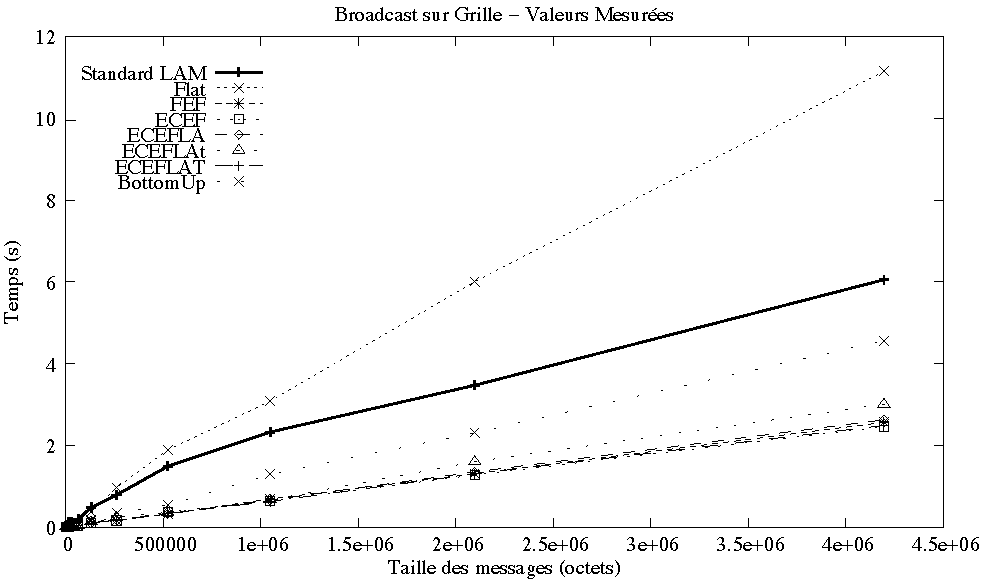
\includegraphics[width=0.7\linewidth]{images/Grid/Bcast/case1/comp}
		\par\end{centering}
	\caption{\label{Figure: Bcast - Case1 - Mesure}Performance du Broadcast sur
		un grid de 88 machines }	
\end{figure}

\begin{figure}[h]
	\begin{centering}
		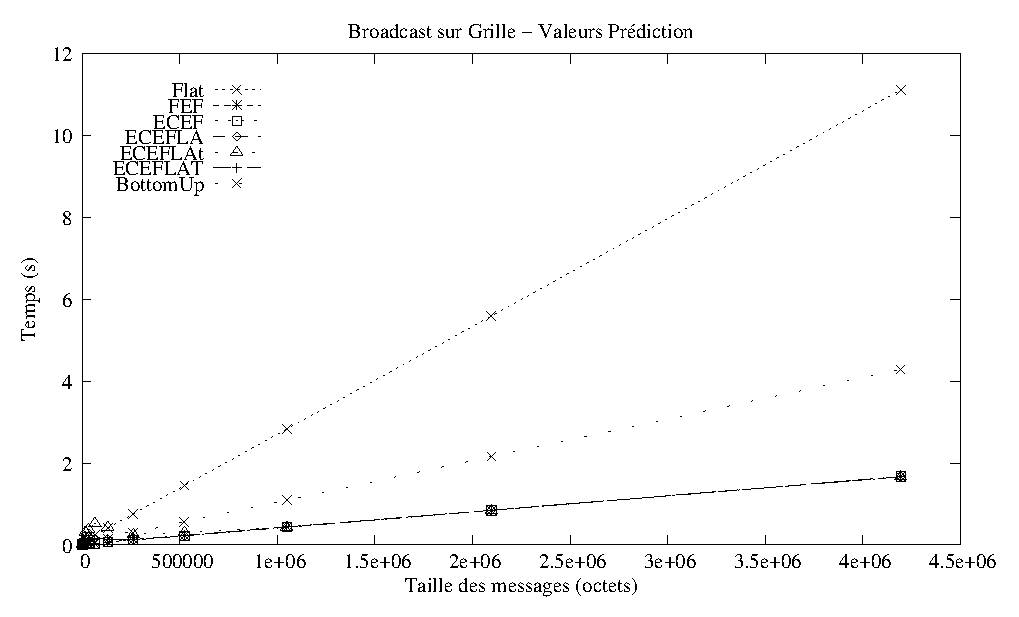
\includegraphics[width=0.7\linewidth]{images/Grid/Bcast/case1/simul}
		\par\end{centering}
	
	\caption{\label{Figure: Bcastcase1predictions}Prédictions pour un grid
		avec 88 machines}
	
\end{figure}

Dans le cas des autres heuristiques, on observe des gains de performance
déjà très importants. L'heuristique BottomUp %, comme prévu par lessimulations, 
n'est pas aussi efficace que les autres heuristiques,
qui de leur côté, se comportent de manière très similaire.

Le faible écart observé entre les prédictions des heuristiques de
type FEF et ECEF-{*} est justifié surtout par le nombre réduit de
clusters, qui réduit le nombre de combinaisons possibles et fait converger
les résultats des différentes heuristiques. 

Pour mieux valider les résultats des expériences, la Figure \ref{Figure: Bcastcase1predictions}
présente les temps prévus des différentes heuristiques. Ces temps,
calculés automatiquement par les heuristiques d'ordonnancement des
communications, donnent une meilleure indication de la fiabilité des
modèles par rapport aux résultats pratiques. Dans ce cas, nous observons
que les heuristiques de type FEF et ECEF-{*} ont des résultats très
rapprochés, certainement parce qu'elles ont obtenu le même ordonnancement
des communications. D'un autre côté, l'écart entre ces prédictions
et les résultats réels sont bien plus importants pour les heuristiques
FEF et ECEF-{*} que pour le BottomUp ou le Flat. Cela indique que
le coût du calcul de l'ordonnancement et le coût de la mise en {\oe}uvre
de ces communications sont les facteurs les plus importants, et reflètent
l'augmentation de complexité d'une communication à couches multiples.

Cette étude met en évidence l'importance
du processus racine et de la répartition des processus sur des différents
clusters sur la performance des stratégies plus simples. En effet,
la performance de la stratégie Flat est fortement liée à l'ordre des clusters, généralement fournie par l'utilisateur.
De surcroît, la stratégie Flat utilise toujours le même ordre de diffusion,
indépendamment du rang du processus racine. Au contraire, les heuristiques
les plus élaborées construisent des arbres de diffusion adaptés à
chaque situation, ce qui rend possible un gain de performance plus
important, surtout quand le rôle de \emph{racine} est alterné entre
plusieurs processus.

D'ailleurs, les simulations indiquent que la performance des stratégies
simples, comme le Flat, supportent très mal l'augmentation du nombre
de clusters interconnectés.  Ainsi, nous croyons que, même si
le grid compte un nombre réduit de clusters, l'utilisation d'une
heuristique un peu plus élaborée, comme par exemple l'heuristique
ECEFLA-T, offre le meilleur rapport coût-bénéfice-robustesse.


\section{Amélioration de la performance de MPI\_AlltoAll sur un grid}

Si les stratégies présentés dans les sections précédentes permettent l'optimisation des communications dans le cadre d'une diffusion MPI\_Bcast, d'autres patrons de communication encore plus couteux sont utilisées par les applications scientifiques. L'une de ces patrons, le \textit{many-to-many}, représente un \emph{échange total} d'informations entre les n{\oe}uds \cite{Christara99}. Plus exactement, chaque processus détient $n$ itens de données différentes de taille $m$, lesquels doivent être distribués entre $n$ processus (le processus inclus).  

Vu la complexité de l'opération, les implémentations MPI de All-to-All généralement utilisent des envois directs entre les processus, ce qui peut occasionner la surcharge des communications et des problèmes liés à la congestion du réseau. De surcroît, l'utilisation de cette approche dans un environnement de type grille doit aussi faire face à l'hétérogénéité des temps de communication entre les n{\oe}uds proches et distants.

\subsection{Définitions}

Soit deux clusters ${\mathcal C}_1$
et ${\mathcal C}_2$ avec respectivement $n_1$ n{\oe}uds et $n_2$ n{\oe}uds.
Un réseau, appelé \textit{backbone}, interconnecte les deux clusters. Nous assumons aussi que l'interface réseau utilisée pour la communication avec un réseau distant est la même utilisée pour la communication avec le réseau local. De ce fait et de la topologie du réseau, les communications inter-cluster ne seront jamais plus rapides que celles effectuées à l'intérieur d'un cluster.

Maintenant supposons qu'une application doit échanger des données entre les machines dans ${\mathcal C}_1$ et ${\mathcal C}_2$ et que pour chaque source, les données à destination des autres machines ne sont pas identiques (mais ont toutes une taille $m$).  Comme résultat, nous devons transmettre l'équivalent à $(n_1+ n_2)^2$ messages différents. Alors que plusieurs bibliothèques MPI libraries  (OpenMPI, MPICH2, etc.) implémentent l'opération \textit{MPI\_AllltoAll} en supposant que les n{\oe}uds se trouvent dans le même réseau et donc que les communications ont le même coût, dans notre cas certains messages sont envoyés entre n{\oe}uds d'un même cluster et d'autres entre n{\oe}uds de réseaux différents. Dans le premier cas, la latence des communications est plus favorables que dans le deuxième, et souvent le même principe s'applique pour le débit du réseau.


\subsection{\label{cluster}Modélisation de la congestion du réseau}

La communication intensive engendrée par les opérations de type \textit{alltoall} peut facilement saturer le réseau ou les destinataires, dégradant ainsi la performance globale de l'opération. Chun \cite{Chun01} a démontré que le coût des communications collectives est souvent dominé par le coût de la congestion du réseau et des subséquentes pertes de paquets.

Malheureusement, plusieurs modèles de communication tels que \cite{Christara99} ou \cite{Pjesivac-Grbovic05} ne prennent pas en compte les impacts potentiels de la congestion. En effet, ces travaux considèrent que l'opération All-to-All n'est qu'une exécution parallèle de plusieurs opérations de type \emph{personalized one-to-many} \cite{Johnsson89}. Cela s'exprime par le modèle de performances linéaire représenté en Equation \ref{eq:1}, où $\alpha$ correspond à la latence de communication entre les processus, $\frac{1}{\beta}$ correspond au débit du lien, $m$ représente la taille des messages en octets et  $n$ correspond au nombre de processus:
\begin{equation}
T=(n-1)\times(\alpha+\beta m)\label{eq:1}
\end{equation}

Comme ce modèle linéaire n'est pas capable de prendre en compte la congestion des communications, certains auteurs tels que Bruck \cite{Bruck97b} et Clement \emph{et al.} \cite{Clement96} suggèrent l'utilisation d'un facteur de ralentissement ()\emph{slowdown factor}) proportionnel au nombre de processus communicants.  Labarta et \emph{al.} \cite{Labarta96} aussi suggère l'utilisation d'un facteur de ralentissement basé sur le nombre de messages en transit car, selon eux, si \emph{m} messages sont prêts à être transmis mais seulement \emph{b} canaux sont disponibles, alors les transmissions sont sérialisées en $\left\lceil \frac{m}{b}\right\rceil $ vagues de communication. 

Une approche légèrement différente a été proposée par Chun \cite{Chun01}, qui associe la congestion à la latence et donc utilise différentes valeurs de latence selon la taille des messages. Cependant, ce modèle ignore le nombre de messages circulant sur un réseau ou un lien, alors et ceci est directement lié au phénomène de la congestion. 

\subsection{Modélisation de la congestion dans un cluster homogène}

Afin de mieux comprendre l'impact de la congestion sur les communications collectives de type All-to-All dans les clusters, nous avons proposé en \cite{Steffenel06b} un modèle où la congestion du réseau est dépendant des caractéristiques de l'environnement physique (interfaces réseaux, liens, switches) mais aussi de la taille des messages. En effet, nous avons observé expérimentalement que les temps de communication varient selon la taille des messages,  et que le facteur de contention  $\gamma$ doit aussi prendre cela en compte. 

Ainsi, notre modèle associe le facteur de contention $\gamma$ de Clement et \textit{al.} \cite{Clement96} avec un nouveau paramètre $\delta$, ce dernier dépendant du nombre de processus et de la taille des messages, comme indiqué ci-dessous. Comme résultat, nous associons deux équations (l'une linéaire, l'autre affine) afin de mieux représenter la performance de communication de MPI\_Alltoall dans un réseau donnée, comme illustré en Figure \ref{Figure: local}.
\begin{equation}
T=\left\{ \begin{array}{lc}
(n-1)\times(\alpha+m\beta)\times\gamma & if\, m<M\\
(n-1)\times((\alpha+m\beta)\times\gamma+\delta)\,\,\,\,\, & if\, m\geq M\end{array}\right.\label{eq:6}\end{equation}

\begin{figure}
	\begin{center}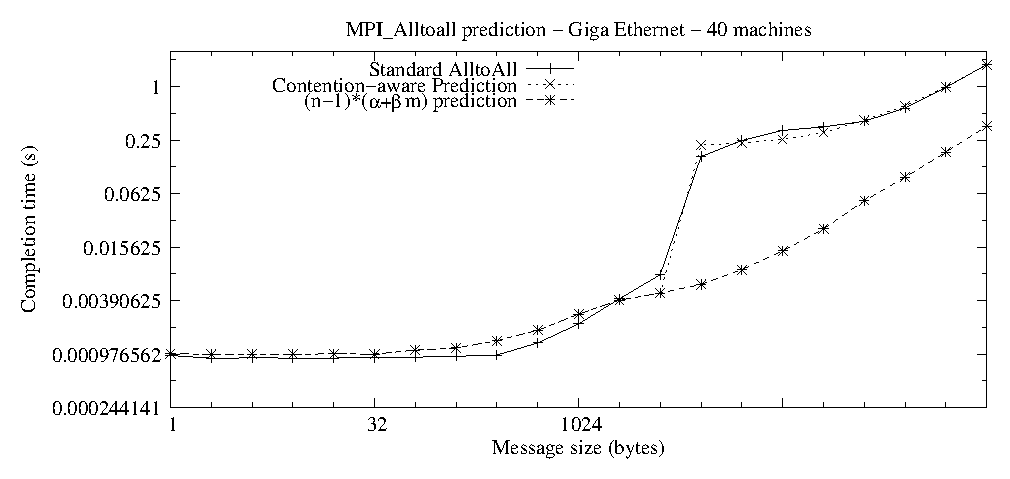
\includegraphics[width=0.7\columnwidth]{images/newcomp24_pred_log}\end{center}
	\caption{\label{Figure: local}Measured and predicted performance for the standard MPI\_Alltoall in a Gigabit Ethernet network}
\end{figure}


Vu la précision de ce modèle pour les clusters homogènes, notre première réaction serait de l'appliquer aussi dans le cas des grids de calcul en faisant la somme des performances des réseaux locaux et distants (Équation \ref{eq:7}). Malheureusement cette stratégie n'aboutit pas car les performances observées sont largement inférieures à celles prévues par ce modèle, comme indique la Figure \ref{Figure: standard}. 

\begin{equation}
T=max(T_{\mathcal C_1},T_{\mathcal C_2})+max(n_1, n_2) \times (\alpha_w+\beta_w \times m)
\label{eq:7}\end{equation}

En effet, la figure \ref{Figure: standard} représente des mesures effectuées entre deux clusters, l'un situé à Nancy et l'autre à Rennes. Les deux clusters étaient constitués de machines similaires (dual Opteron 246, 2 GHz) interconnectées localement par un réseau Gigabit Ethernet, alors que le lien inter-cluster était un réseau privé de 10 Gbps. Les mesures ont été obtenues selon la méthode \emph{broadcast-barrier} \cite{Supinski99}.


\begin{figure}
	\begin{center}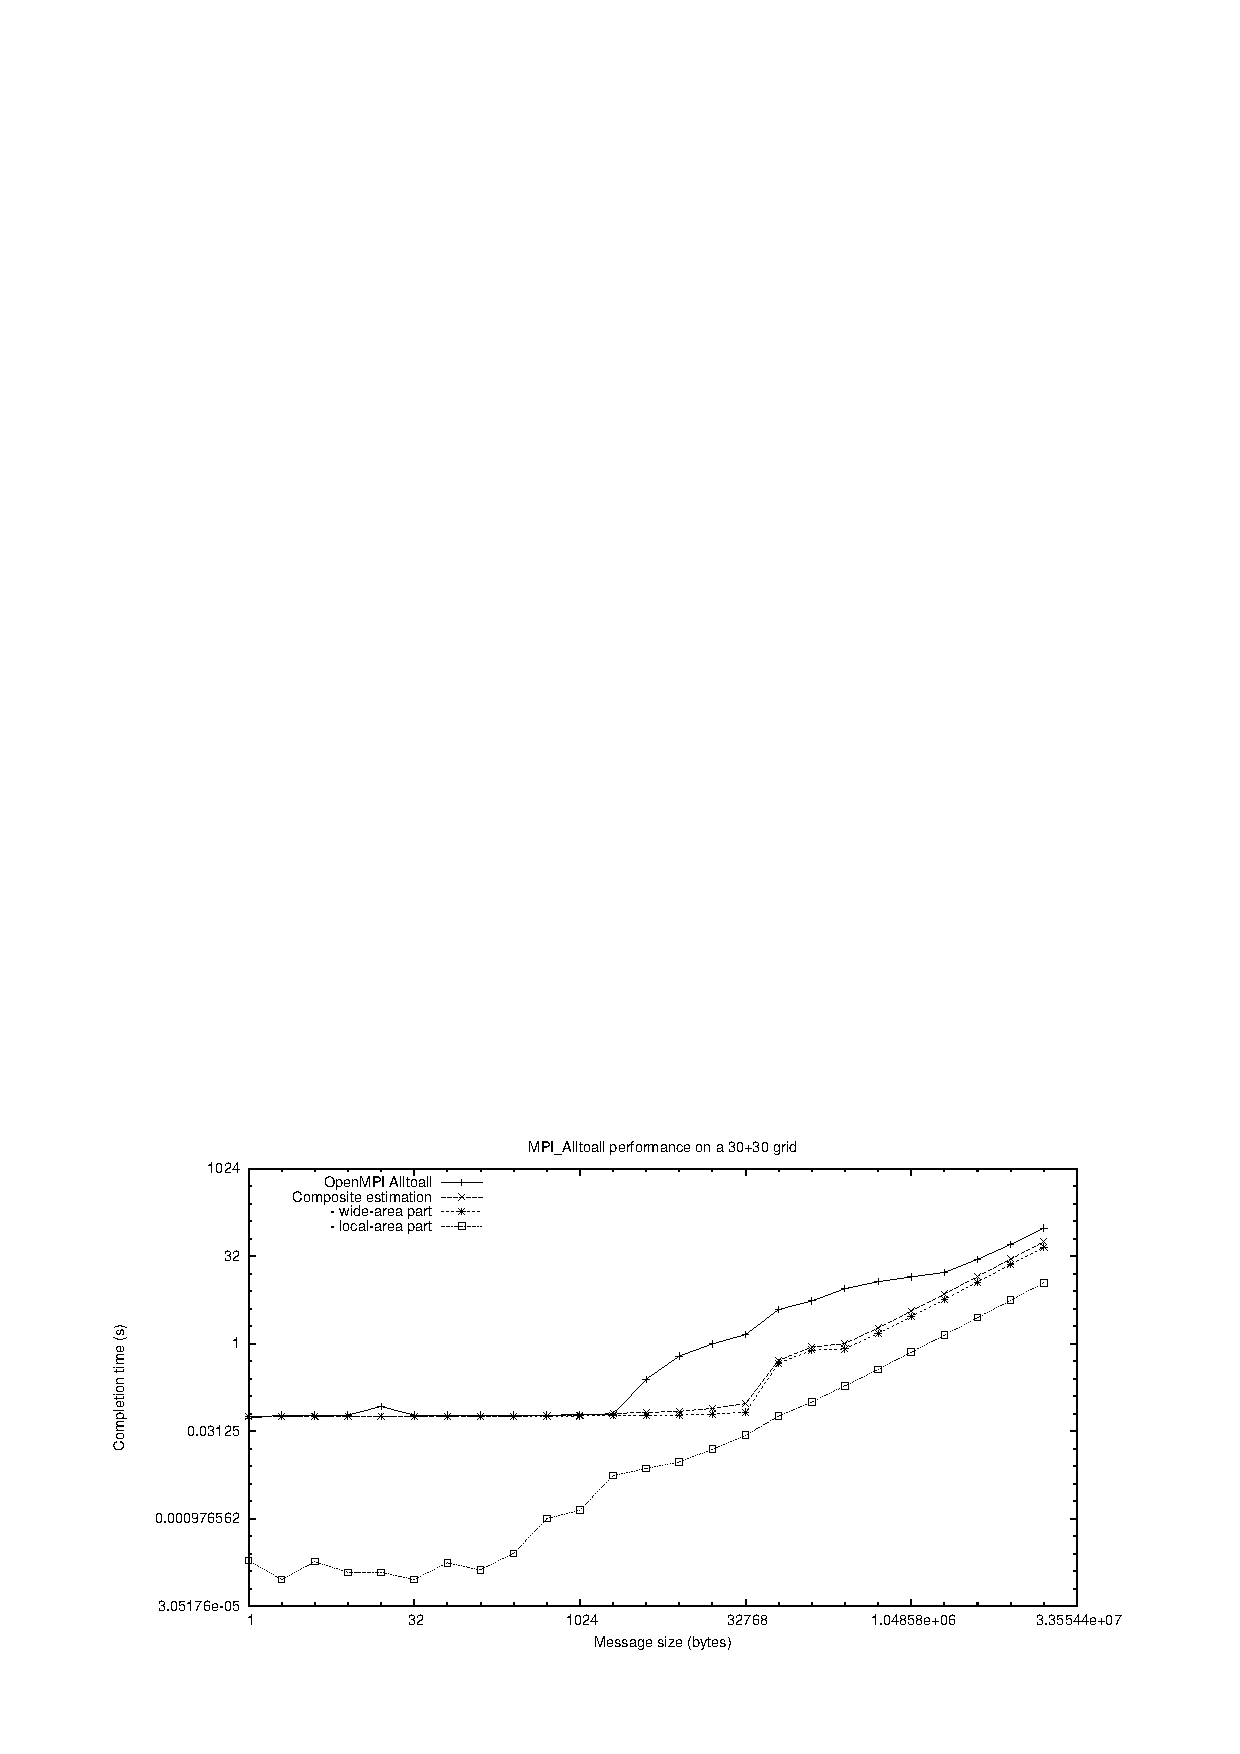
\includegraphics[width=0.7\columnwidth]{images/standard}\end{center}
	\vspace{-0.5cm}\caption{\label{Figure: standard}Measured and predicted performance for the standard MPI\_Alltoall in a grid}\vspace{-0.5cm}
\end{figure}
 
Bien qu'on pourrait rajouter des paramètres supplémentaires pour s'approcher des performances observées, nous avons décidé d'attaquer le problème directement à sa source en optimisant la façon dont les communications sont effectuées sur un grid. 


\subsection{L'algorithme LG}

Lors de l'opération dans un grid de calcul, l'un des facteurs les plus importants à prendre en compte est le temps nécessaire à ce que les messages soient livrés car ceux-ci sont affectés par la distance géographique mais aussi par l'hétérogénéité des protocoles, le routage des messages et les interférences des autres flux rencontrés sur le backbone. 

La plupart des algorithmes pour les communications collectives sur les grids (PACX MPI~\cite{Gabriel98}, MagPIe~\cite{Kielmann01}) visent la minimisation des communications à grande distance en choisissant un coordinateur dans chaque cluster qui sera responsable par les échanges intra-cluster. Bien que ce mécanisme présente des avantages pour d'autres patrons de communication, il n'est pas adapté aux opérations de type  MPI\_Alltoall. En premier lieu, ce mécanisme  induit des étapes de communication supplémentaires du fait de forcer le passage par les coordinateurs des clusters, qui de plus deviennent des goulots d'étranglement. En deuxième lieu, cette approche n'est pas optimale par rapport à l'utilisation des liens inter-cluster, souvent capables de supporter des flux multiples \cite{Casanova05}. 

Afin de mieux traiter ce problème, nous essayons de minimiser les échanges distants d'une autre manière. En effet, la grande complexité des échanges du All-to-All réside dans les différentes perforances des liens locaux et distants, or les implémentations traditionnelles de MPI\_Alltoall sont incapables de faire la différence. Si nous pouvons identifier la disposition des n{\oe}uds, on peut utiliser toutes les machines d'un cluster pour collecter les données à un niveau local avant de les envoyer simultanément au réseau distant, en une unique étape de communication. 

Ainsi, le mécanisme que nous avons proposé en \cite{Steffenel07c} est une solution "grid aware" qui s'exécute en deux étapes. Dans un premier moment, seulement les échanges locaux sont effectués. Cette phase inclut les échanges attendus entre les n{\oe}uds intra-cluster mais aussi l'échange des données destinés aux autres clusters, stockés dans des buffers supplémentaires pour la deuxième phase. L'avantage de cet échange est que son coût est très faible par rapport au coût d'une communication distante (voir Figure \ref{Figure: standard}). Finalement, lors de la deuxième phase, les buffers sont transmis directement aux n{\oe}uds destinataires, complétant ainsi l'échange total.  

Plus exactement, l'algorithme peut être décrit comme suit. Sans perte de généralité, considérons un cluster  ${\mathcal C}_1$ qui contient moins de n{\oe}uds que le cluster ${\mathcal C}_2$ ($n_1\leq n_2$). Les n{\oe}uds sont ainsi numérotés de 0 à $n_1+n_2-1$, avec les n{\oe}uds allant de 0 à $n_1-1$ appartenant à ${\mathcal C}_1$ et les n{\oe}uds allant de $n_1$ à $n_1+n_2-1$ appartenant au cluster ${\mathcal C}_2$. Nous appelons ainsi ${\mathcal M}_{i,j}$ le message (donnée) qui sera envoyé du n{\oe}ud $i$ au n{\oe}ud $j$. 

L'algorithme suit les deux étapes : 
\begin{description}
	\item[Première étape] Pendant cette phase, nous effectuons les échanges locaux : Le processus $i$  envoie ${\mathcal M}_{i,j}$ au processus $j$, seulement si $i$ et $j$ font partie du même cluster. Ensuite, ils préparent les buffers pour les communications distantes de manière à ce que les données à destination d'un node distant $j$ on ${\mathcal C}_2$ seront d'abord stockés sur le n{\oe}ud $j~ mod~ n_1$ de ${\mathcal C}_1$. De même, les données sur un n{\oe}ud $i$ de ${\mathcal C}_2$ à destination de $j$ sur ${\mathcal C}_1$ seront stockés sur le n{\oe}ud $ \lfloor i/n_1 \rfloor \times n_1 + j $.
	\item[Deuxième étape] Pendant cette deuxième étape, seulement $n_2$ communications inter-cluster auront lieu. Cette phase est décomposée en $\lceil n_2/n_1\rceil$ vagues avec $n_1$ communications chacune. Ainsi, pendant la vague $s$, le processus  $i$ de ${\mathcal C}_1$ échangera son buffer local avec le processus $j=i+n_1\times s$ de ${\mathcal C}_2$ (si $j < n_1+n_2$). Plus exactement, $i$ envoie  ${\mathcal M}_{k,j}$ à $j$ où $k\in [0,n_1]$ et $j$ envoie ${\mathcal M}_{k,i}$ à $i$ où $k\in[n_1\times s,n_1\times s+n_1-1]$.
\end{description}

Comme cet algorithme minimise le nombre de communications inter-cluster et les organise par vagues, nous n'avons besoin que de $2\times \max(n_1,n_2)$ messages dans les deux directions (par rapport à  $2\times n_1 \times n_2$ messages dans l'algorithme traditionnel). Si les deux clusters ont le même nombre de n{\oe}uds, une seule vague d'échanges sera nécessaire. Notre algorithme est aussi optimisé sur la longue distance car il regroupe plusieurs messages ensemble, réduisant l'impact de la latence et des interférences sur le backbone. La Figure \ref{Figure: comp} présente une comparaison entre la performance de l'algorithme traditionnel implémenté par OpenMPI et celle de l'implémentation de l'algorithme ${\mathcal LG}$. Nous observons que l'algorithm ${\mathcal LG}$ obtient un gain de performance de presque 50\% par rapport à la stratégie traditionnelle.

\begin{figure}
	\begin{center}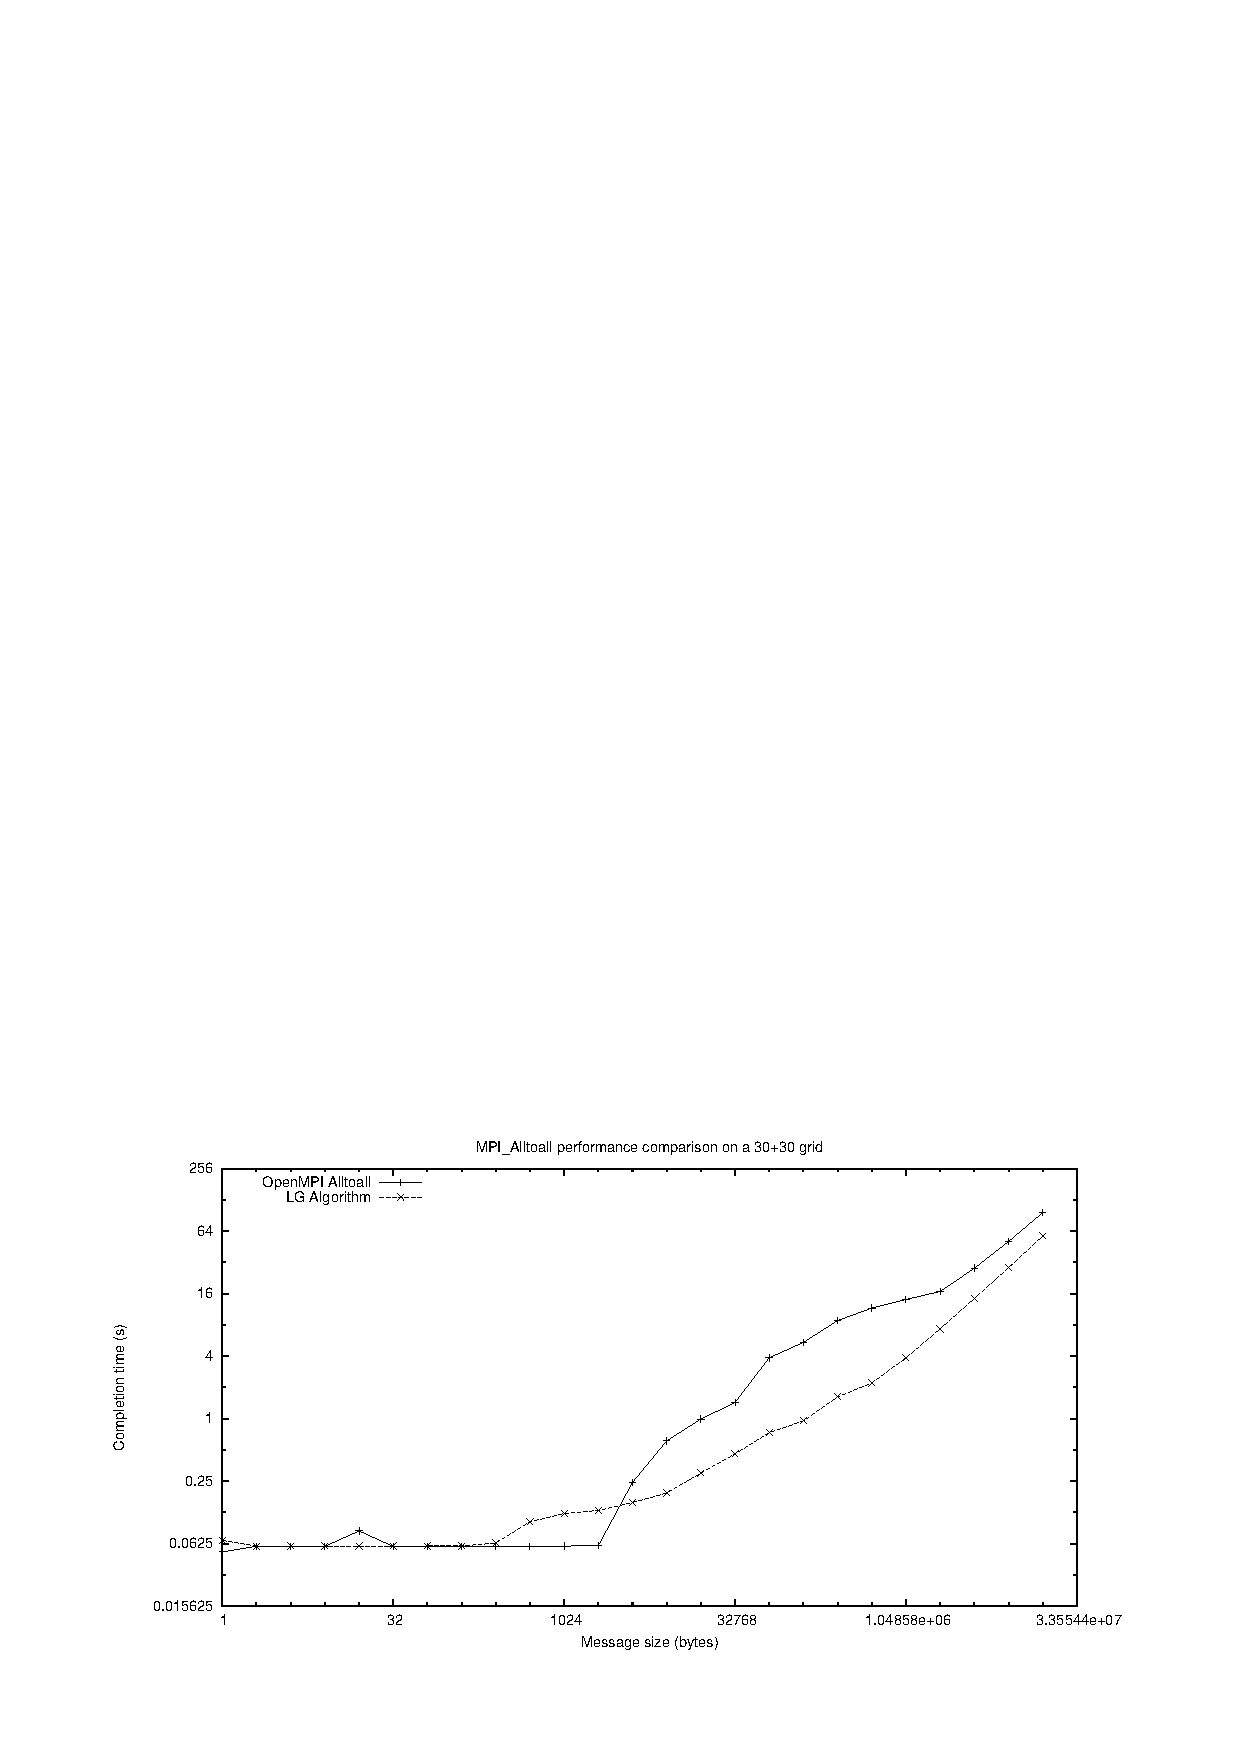
\includegraphics[width=0.7\columnwidth]{images/comp}\end{center}
	\caption{\label{Figure: comp}Comparaison de performance entre OpenMPI et ${\mathcal LG}$ algorithms}
\end{figure}

L'ordonnancement des communications effectué par ${\mathcal LG}$ a aussi une conséquence sur la modélisation des performances. Tout d'abord, il minimise les communications de longue distance, réduisant les risques de congestion qui sont difficiles de modéliser. De plus, la transmission groupée des messages réduit l'impact de la latence et des fluctuations de performance du réseau. C'est ainsi que nous avons pu établir un modèle composé des performances locales (${\mathcal T_{C_{n}}}$, obtenues à partir de l'équation \ref{eq:6}) et des prédictions pour les communications de longue distance obtenues par les méthodes traditionnelles :

\begin{equation}
T=max(T_{\mathcal C_1},T_{\mathcal C_2})+\lceil n_2/n_1\rceil \times (\alpha_w+\beta_w \times m \times n_1)
\label{eq:8}\end{equation}

Afin d'obtenir les paramètres nécessaires aux prédictions, nous avons utilisé la procédure décrite par Kielman \textit{et al.} \cite{Kielmann00}. Les facteurs de contention $\gamma=2.6887$ et $\delta=0.005039$ pour $M>=1KB$ ont été obtenus par la méthode des moindres carrés comme décrit par \cite{Steffenel06b}.

\begin{figure}
	\begin{center}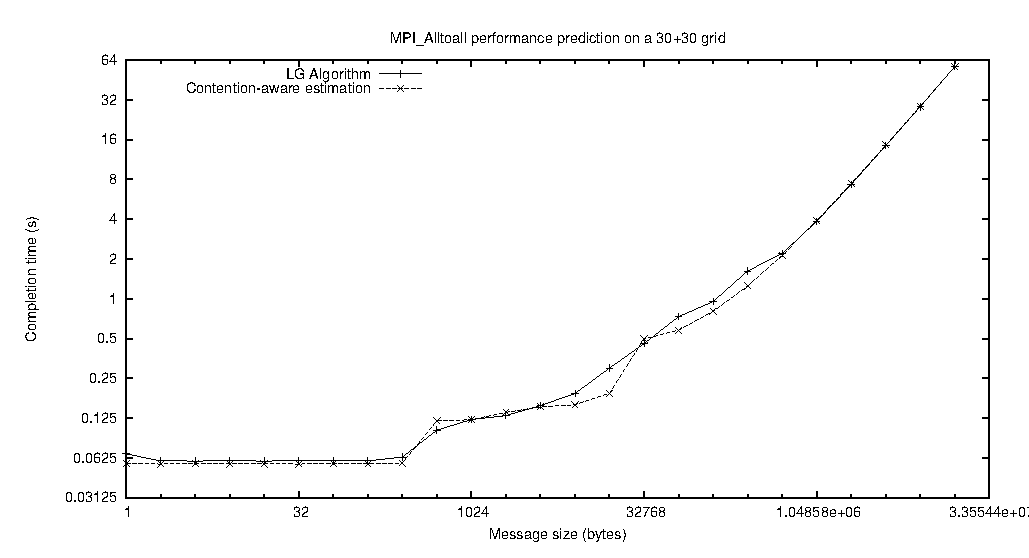
\includegraphics[width=0.7\columnwidth]{images/simul}\end{center}
	\caption{\label{Figure: simul}Performance de ${\mathcal LG}$ et sa prédiction}
\end{figure}

La Figure \ref{Figure: simul} compare ainsi les prédictions obtenues avec l'Equation \ref{eq:8} et les performances mesurées pour l'algorithm ${\mathcal LG}$. Nous observons une bonne adéquation des prédictions, ce qui était impossible avec l'implémentation traditionnelle de MPI\_Alltoall. 

\section{Bilan et Perspectives}

Dans ce chapitre nous avons présenté une stratégie efficace pour identifier
et découper les réseaux en clusters logiques homogènes. La présence
des hétérogénéités réduit la précision des modèles de communication
utilisés pour optimiser les communications collectives. Le \emph{framework}
proposé réussi à obtenir des paramètres de connectivité par un coût
très faible, à partir du regroupement d'informations obtenues indépendamment
dans chaque cluster. Notre approche, validée par des tests pratiques,
démontre que la découverte de topologie peut se faire de façon rapide
et précise. Associé à des modèles de prédiction de performance, le
découpage des clusters s'avère essentiel à l'optimisation des primitives
de communication collective, spécialement pour celles structurées
en multiples couches. De plus, ce \emph{framework} peut être étendu,
de manière à détecter aussi la présence de machines multiprocesseur,
information importante pour l'optimisation des communications.

